\chapter{Finite automata minimization algorithms}

\section{Introduction}

\section{Brzozowski's algorithm}

\begin{flushleft}
$\epsilon-free$ FA: $M_0=(Q_0,V,T_0,\emptyset,S_0,F_0)$ \\
to be minimized $DFA$: $M_2=(Q_2,V,T_2,\emptyset,S_2,F_2)$ \\
intermediate $NFA$: $M_1=(Q_1,V,T_1,\emptyset,S_1,F_1)$\\
\end{flushleft}

NFA: $M_1 \to $ DFA: $M_2, M_2=suseful_s\circ subsetopt(M_1)$
\begin{align*}
& q_0,q_1\in Q_1,Q_2\subseteq\mathbb{P}(Q_1),\forall p\in  Q_2,p=(q_0,q_1)\\
& \overrightarrow{L}_{M_2}(p)=\overrightarrow{L}_{M_1}(q_0)\cup  \overrightarrow{L}_{M_1}(q_1)\\
& \Rightarrow \\
& \overrightarrow{L}_{M_2}(p)=\bigcup_{q\in p}\overrightarrow{L}_{M_1}(q)\\
& \Rightarrow 
\end{align*}

\begin{figure}[htbp]
	\begin{tikzpicture}
	\matrix (a) [matrix of math nodes,row sep=3em,
	column sep=5em, nodes in empty cells]
	{ Q_1 &  P(Q_1) \\ 
		&  D(Q_2) \\};
	\path[>=latex,->] 
	(a-1-1) edge node [auto] {$subsetopt$} (a-1-2)
	edge node [auto,swap] {$$} (a-2-2)
	(a-1-2) edge node [auto] {$useful_s$} (a-2-2)
	;
	\end{tikzpicture}
	\caption{$M_2=suseful_s\circ subsetopt(M_1)$}
\end{figure}

\begin{figure}[htbp]
	\subfigure[$M_1=(Q_1,V,T_1,\emptyset,S_1,F_1)$] { \label{fig:a} 
	\begin{tikzpicture}[->,>=stealth',shorten >=1pt,auto,node distance=2cm, semithick]
		\tikzstyle{every state}=[minimum size=0.1mm]
		\node[state] (q)  [] {$q$};
		\node[state] (q0) [above right of=q] {$q_0$};
		\node[state] (q1) [below right of=q] {$q_1$};
		\node[state] (f1)  [below right of=q0] {$f_1$};
		\path 
		(q) edge [] node {$a$} (q0)
		    edge [swap] node {$a$} (q1)
		(q0) edge [] node {$\overrightarrow{L}_{M_1}(q_0)$} (f1)
		(q1) edge [swap] node {$\overrightarrow{L}_{M_1}(q_1)$} (f1)
		;
	\end{tikzpicture}
    }
    \hspace{2cm}
	\subfigure[$M_2=(Q_2,V,T_2,\emptyset,S_2,F_2)$] { \label{fig:b}
    \begin{tikzpicture}[->,>=stealth',shorten >=1pt,auto,node distance=3cm, semithick,scale=4]
    	\tikzstyle{every state}=[minimum size=0.1mm]
    	\node[state] (q01)  {$(q_0,q_1)$};
    	\node[state] (f2)  [right of=q01] {$f_2$};
    	\path 
    	(q01) edge [bend left] node {$\overrightarrow{L}_{M_1}(q_0)$} (f2)
    	(q01) edge [bend right,swap] node {$\overrightarrow{L}_{M_1}(q_1)$} (f2)
    	;
    \end{tikzpicture}
    }
	\caption{$M_2=suseful_s\circ subsetopt(M_1)$}
\end{figure}

\begin{figure}[htbp]
	\subfigure[$M_0=(Q_0,V,T_0,\emptyset,S_0,F_0)$] {
		\begin{tikzpicture}[->,>=stealth',shorten >=1pt,auto,node distance=2cm, semithick]
		\tikzstyle{every state}=[minimum size=0.1mm]
		\node[state,accepting] (q2) []{$q_2$};
		\node[state,initial] (q0) [above left of=q2] {$q_0$};
		\node[state] (q1) [above right of=q2] {$q_1$};
		\path
		(q0) edge[bend left] node {$0$} (q1)
		(q1) edge[bend left] node {$0$} (q0)
		(q0) edge[swap] node {$1$} (q2)
		(q1) edge[] node {$1$} (q2)
		(q2) edge[loop below] node {$0,1$} (q2)
		;
		\end{tikzpicture}
	}
    \hspace{1cm}
	\subfigure[$M^R_0=(Q_0,V,T_0,\emptyset,S_0,F_0)^R=(Q_0,V,T^R,\emptyset,F_0,S_0)$]{
		\begin{tikzpicture}[->,>=stealth',shorten >=1pt,auto,node distance=2cm, semithick]
		\tikzstyle{every state}=[minimum size=0.1mm]
		\node[state,initial] (q2) []{$q_2$};
		\node[state,accepting] (q0) [above left of=q2] {$q_0$};
		\node[state] (q1) [above right of=q2] {$q_1$};
		\path
		(q1) edge[bend right,swap] node {$0$} (q0)
		(q0) edge[bend right,swap] node {$0$} (q1)
		(q2) edge[] node {$1$} (q0)
		(q2) edge[swap] node {$1$} (q1)
		(q2) edge[loop below] node {$0,1$} (q2)
		;
		\end{tikzpicture}
	}
    \newline
	\subfigure[$useful_s\circ subsetopt\circ R(M_0)$]{
		\begin{tikzpicture}[->,>=stealth',shorten >=1pt,auto,node distance=2cm, semithick]
		\tikzstyle{every state}=[minimum size=0.1mm]
		\node[state,initial] (q2) []{$q_2$};
		\node[state,accepting] (q0) [above of=q2] {$\{q_0,q_1,q_2\}$};
		\path
		(q2) edge[] node {$1$} (q0)
		(q0) edge[loop above] node {$0,1$} (q0)
		(q2) edge[loop below] node {$0$} (q2)
		;
	\end{tikzpicture}
	}
    \hspace{3cm}
    \subfigure[$M_1=R\circ useful_s\circ subsetopt\circ R(M_0)$]{
    	\begin{tikzpicture}[->,>=stealth',shorten >=1pt,auto,node distance=2cm, semithick]
    	\tikzstyle{every state}=[minimum size=0.1mm]
    	\node[state,accepting] (q2) []{$q_2$};
    	\node[state,initial] (q0) [above of=q2] {$\{q_0,q_1,q_2\}$};
    	\path
    	(q0) edge[] node {$1$} (q2)
    	(q0) edge[loop above] node {$0,1$} (q0)
    	(q2) edge[loop below] node {$0$} (q2)
    	;
    	\end{tikzpicture}
    }
    \caption{$M_1=R\circ useful_s\circ subsetopt\circ R(M_0)$}
\end{figure}

\begin{figure}[htbp]
	\begin{align*}
	\text{start: } &U=\{q_2\},D=\emptyset \\
	u=q_2: & T(q_2,0)=\{q_2\},T(q_2,1)=\{q_0,q_1,q_2\} \\
	&\text{add new state to $D$, } D=\{q_2,\{q_0,q_1,q_2\}\} \\
	u=\{q_0,q_1,q_2\}:& T(\{q_0,q_1,q_2\},0)=T(q_0,0)\cup T(q_1,0)\cup T(q_2,0)=\{q_1\}\cup \{q_0\}\cup \{q_2\} =\{q_0,q_1,q_2\}\\
	&T(\{q_0,q_1,q_2\},1)=T(q_0,1)\cup T(q_1,1)\cup T(q_2,1)=\emptyset\cup \emptyset \cup \{q_0,q_1,q_2\}=\{q_0,q_1,q_2\}
	\end{align*}
	
	\subfigure[$M$]{
		\begin{tikzpicture}[->,>=stealth',shorten >=1pt,auto,node distance=2cm, semithick]
		\tikzstyle{every state}=[minimum size=0.1mm]
		\node[state,initial] (q2) []{$q_2$};
		\node[state,accepting] (q0) [above left of=q2] {$q_0$};
		\node[state] (q1) [above right of=q2] {$q_1$};
		\path
		(q1) edge[bend right,swap] node {$0$} (q0)
		(q0) edge[bend right,swap] node {$0$} (q1)
		(q2) edge[] node {$1$} (q0)
		(q2) edge[swap] node {$1$} (q1)
		(q2) edge[loop below] node {$0,1$} (q2)
		;
		\end{tikzpicture}
	}
    \hspace{2cm}
	\subfigure[$useful_s\circ subsetopt(M)$]{
		\begin{tikzpicture}[->,>=stealth',shorten >=1pt,auto,node distance=2cm, semithick]
		\tikzstyle{every state}=[minimum size=0.1mm]
		\node[state,initial] (q2) []{$q_2$};
		\node[state,accepting] (q0) [right of=q2] {$\{q_0,q_1,q_2\}$};
		\path
		(q2) edge[] node {$1$} (q0)
		(q0) edge[loop above] node {$0,1$} (q0)
		(q2) edge[loop above] node {$0$} (q2)
		;
		\end{tikzpicture}
	}
	\caption{$useful_s\circ subsetopt(M)$}
\end{figure}

\section{Minimization by equivalence of states}

\begin{figure}[htbp]
	Equivalence relation $E\subseteq Q\times Q$\\
	$(p,q)\in E\equiv (\overrightarrow{L}(p)=\overrightarrow{L}(q))$\\
	
	\subfigure[$(p,q)\in E$]{
		\begin{tikzpicture}[->,>=stealth',shorten >=1pt,auto,node distance=2cm, semithick]
		\tikzstyle{every state}=[minimum size=0.1mm]
		\node[state,accepting] (f) {$f$};
		\node[state] (p) [above left of=f]{$p$};
		\node[state] (q) [below left of=f]{$q$};
		\path
		(p) edge[] node {$\overrightarrow{L}(p)$} (f)
		(q) edge[swap] node {$\overrightarrow{L}(q)$} (f)
		;
		\end{tikzpicture}
		}
	    \hspace{2cm}
    	\subfigure[$(p,q)\in E$]{
    	\begin{tikzpicture}[->,>=stealth',shorten >=1pt,auto,node distance=2cm, semithick]
    	\tikzstyle{every state}=[minimum size=0.1mm]
    	\node[state,accepting] (f) {$f$};
    	\node[state] (p) [left of=f]{$[p,q]$};
    	\path
    	(p) edge[] node {$\overrightarrow{L}(\#)$} (f)
    	;
    	\end{tikzpicture}
   		}
	\caption{Equivalence relation $E\subseteq Q\times Q$}
\end{figure}

\begin{figure}[htbp]
	$\overrightarrow{L}(p)=\bigcup_{a\in V}(\{a\} \cdot \overrightarrow{L}(T(p,a)) \cup \{\epsilon|p\in F\}$\\

	\begin{tikzpicture}[->,>=stealth',shorten >=1pt,auto,node distance=3cm, semithick]
		\tikzstyle{every state}=[minimum size=0.1mm]
		\node[state,accepting] (p) {$p$};
		\node[state] (q1) [above right of=p]{$T(p,a)$};
		\node[state] (q2) [below right of=p]{$T(p,b)$};
		\node[state,accepting] (f1) [right of=q1]{$f1$};
		\node[state,accepting] (f2) [right of=q2]{$f2$};
		\path
		(p) edge[] node {$a$} (q1)
		(p) edge[] node {$b$} (q2)
		(q1) edge[] node {$\overrightarrow{L}(T(p,a))$} (f1)
		(q2) edge[] node {$\overrightarrow{L}(T(p,b))$} (f2)
		;
	\end{tikzpicture}
	\caption{$L(p)$}
\end{figure}

Let $A=(Q,V,T,_,F)$ be a deterministic finite automaton, where $Q$ is a finite set of states, $V$ is a finite set of input symbols, $T$ is a mapping from $Q\times V$ into $Q$, and $F\subseteq Q$ is the set of final states. No initial state is specified since it is of no importance in what follows. The mapping $T$ is extended to $T\times V^\ast$ in the usual manner where $V^\ast$ denotes the set of all finite strings (including the empty string $\epsilon$) of symbols from $V$

\begin{definition}[equivalent states]
	The states $s$ and $t$ are said to be equivalent if for each $x\in V^\ast, T(s,x)\in F$ if and only if $T(t,x)\in F$. 
\end{definition}

\begin{figure}[htbp]
	a: $((T(p,a),T(q,a))\in E_0$; b: $((T(p,a),T(q,a))\notin E_0$, c: $((T(p,a),T(q,a))\in E_1(part_1)$; d: $((T(p,a),T(q,a))\notin E_1(part_1)$;\\
	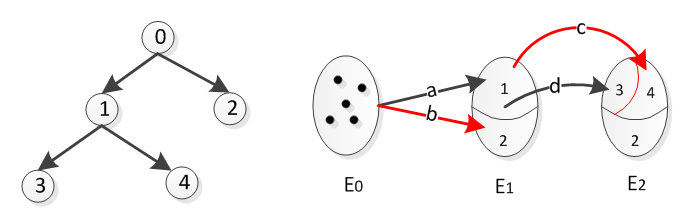
\includegraphics[scale=0.8]{approximatingE}
	\caption{Approximating $E, E_0=(Q\setminus F)^2\cup F^2$ }
\end{figure}

\begin{figure}[htbp]
	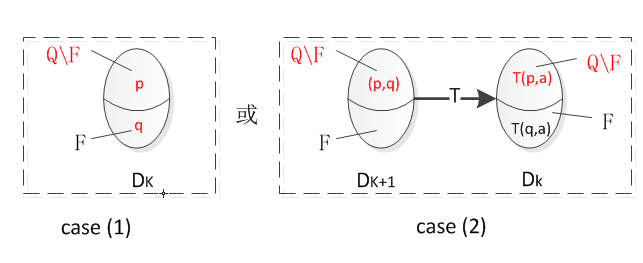
\includegraphics[scale=0.8]{approximatingD}
	\caption{Approximating $D, D_0=((Q\setminus F)\times F)\cup (F\times (Q\setminus F))$ }
\end{figure}

\begin{figure}[htbp]
	initial,$P=[Q]_{E_0}=\{F,Q\setminus F\},Q_0,Q_1\in P$, \\
	if ($\exists p,q\in Q_0,T(p,a)\in Q_1$, and  $T(q,a)\notin Q_1$), then \\
	split $Q_0$ (wrt $Q_1$) $\to$ two parts, (1): $Q_0^\prime\in Q_1$ and (2): $(Q_0\setminus Q_0^\prime)\notin Q_1$ \\
	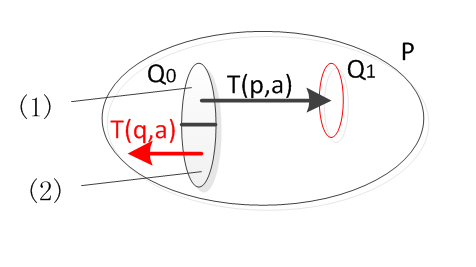
\includegraphics[scale=0.8]{splittable}
	\caption{split $Q_0$ wrt $Q_1$ }
\end{figure}

\section{From \cite{Gries73}}

\subsection{Problem Definition}

DFA: $A=(S,I,\delta,F)$, No initial state is specified since it is of no importance in what follows.

\begin{definition}[equivalent states]
	States $s$ and $t$ are said to be equivalent if for each $x\in I^\ast,\delta(s,x)\in F$. if and only if $\delta(t,x)\in F$.
\end{definition}

We want an algorithm which finds equivalent states of a finite automaton.

\begin{example}
	Consider the automaton with $S=\{a,b,c,d,e\},I=\{0,1\},F=\{d,e\}$ and $\delta$ is given by the arc of diagram of Fig. \ref{fig:ex}.
\begin{figure} [htbp]
	\{a,b\},\{d,e\}is not equivalent states. \\
	Sets of equivalent states: \{a,c\},\{b\},\{d\},\{e\}\\
	%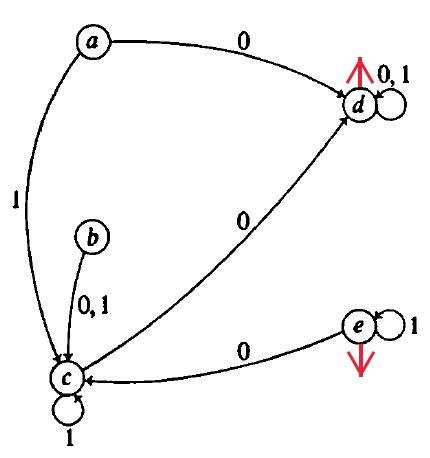
\includegraphics[scale=0.4] {mini-fa} 
	\begin{tikzpicture}[->,>=stealth',shorten >=1pt,auto,node distance=1.5cm, semithick]
	\tikzstyle{every state}=[minimum size=0.1mm]
	\node[state] (a) {$a$};
	\node[state,accepting] (d) [right of=a] {$d$};
	\node[state] (c) [below of=a] {$c$};
	\node[state] (b) [left of=c] {$b$};
	\node[state,accepting] (e) [right of=c] {$e$};
	\path
	(d) edge [loop above] node {$0,1$} (d)
	(c) edge [loop below] node {$1$} (c)
	(e) edge [loop below] node {$1$} (e)
	(a) edge [] node {$0$} (d)
	(a) edge [swap] node {$1$} (c)
	(b) edge [swap] node {$0,1$} (c)
	(e) edge [] node {$0$} (c)
	(c) edge [] node {$0$} (d)
	;
	\end{tikzpicture}
	\caption{Finite state automaton}
	\label{fig:ex}
\end{figure}
\end{example}

\subsection{The Basic Algorithm}
\begin{definition}[acceptable partition]
	A partitioning of the states into blocks $B_1,B_2,\dots,B_p$ is acceptable if (a) no block contains both a final and a nonfinal state, and (b) if $s$ and $t$ are equivalent states then they are in the same block.
\end{definition}

\begin{lemma} \label{lem:partitioning}
	The partitioning $B_1=F,B_2=S-F$ is acceptable.
\end{lemma}

\begin{lemma} \label{lem:stSame}
	The partitioning $B_1,B_2,\dots,B_p$ gives the blocks of equivalent states if and only if (a) the partitioning is acceptable and (b) for each pair of blocks $B_i,B_j$ and symbol $a\in I$
	\begin{equation}
	s,t\in B_i,\delta(s,a)\in B_j \text{ implies } \delta(t,a)\in B_j
	\end{equation}
\end{lemma}

\begin{lemma} \label{lem:split}
	Let $B_1,B_2,\dots,B_p$ be an acceptable partitioning. Suppose there are two blocks $B_i,B_j$ and symbol $a\in I$ such that
	\begin{equation}
	s,t\in B_i,\delta(s,a)\in B_j \text{ but } \delta(t,a)\notin B_j
	\label{eq:split}
	\end{equation}
	
	Then $s$ and $t$ are not equivalent states, and we get a new acceptable partitioning by replacing $B_i$ by the two blocks
	\begin{equation}
	\{s\in B_i|\delta(s,a)\in B_j\} \text{ and } \{s\in B_i|\delta(s,a)\notin B_j\}
	\end{equation}
\end{lemma}

This splitting of $B_i$ as described is called splitting $B_i$ with respect to the pair $(B_i, a)$ or simply splitting $B_i$ wrt $(B_j, a)$. We now write the following algorithm:

\begin{algorithm}  
	\caption{splitting $B_i$ wrt $(B_j, a)$} 
	\label{alg:splitting} 
	\begin{algorithmic}%[1] %每行显示行号
	\State $B_1 \gets F; B_2\gets S-F;$  [initially there are two blocks]  
	\While { $\exists a,B_i,B_j $ such that Eq. (\ref{eq:split}) holds }
		\State SPLIT: split $B_i$ wrt $(B_j,a)$
	\EndWhile
	\end{algorithmic}   
\end{algorithm}

$B$,$P$ are relations, $S$ is a sequence of statements.
\begin{equation}
	P\land B\{S\}P \text{ implies $P$ \{While $B$ do $S$ end\} } P\land\lnot B
\end{equation}

For algorithm (\ref{alg:splitting}), let $P$ be the relation ``the partitioning is acceptable". By Lemma \ref{lem:partitioning}, $P$ is true just before execution of the while loop, while by Lemma \ref{lem:split} execution of $S$ always yields an acceptable partitioning. The relation $B$ is ``$\exists a,B_i,B_j such that  Eq. (\ref{eq:split}) holds $". Thus, $P$ and $\lnot B$ hold after execution of the loop, but these are the sufficient requirements described in Lemma \ref{lem:stSame} for the final partitioning to be the described one.

Our refinement (\ref{alg:refinement}) determines all splittings wrt a pair $(B_i, a)$ and then performs all these splittings at the same time.
\begin{algorithm}  
	\caption{splitting $B_i$ wrt $(B_j, a)$} 
	\label{alg:refinement} 
	\begin{algorithmic}%[1] %每行显示行号
		\State $B_1 \gets F; B_2\gets S-F;$  [initially there are two blocks]  
		\While { $\exists a,B_i,B_j $ such that Eq. (\ref{eq:split}) holds }
		\State Determine the splittings of all blocks wrt $(B_j,a)$
		\State Split each block as just determined.
		\EndWhile
	\end{algorithmic}   
\end{algorithm}

The algorithm is not very efficient, it's $|I||S|^2$.

The result of splitting all blocks wrt $(B_j, a)$ is that any future block $B$ (including the final blocks) satisfies one of the following:

\begin{align}
&\text{(a) for all } s\in B\quad \delta(s,a)\in B_j, \text{ or } \label{eq:splitB} \\
&\text{(b) for all } s\in B\quad \delta(s,a)\notin B_j \notag %无编号
\end{align}

\begin{lemma} 
	Suppose all blocks have been split wrt $(B_j, a)$. Then there is no need to split any future block wrt $(B_j, a)$.
\end{lemma}

\begin{lemma} \label{lem:three_pairs}
Suppose a block $B_j$ is split into blocks $\bar{B}_j$ and $\tilde{B}_j$. Consider a symbol $a$. Splitting all blocks wrt to any two of the three pairs $(B_j, a), (\bar(B)_j, a)$, and $(\tilde{B}_j, a)$ performs the same function as splitting all blocks wrt all three pairs.
\end{lemma}

\begin{proof}
	Suppose we split all blocks wrt $(B_j, a)$ and $(\bar{B}_j, a)$. This implies that each future block $B$ satisfies one of the following:
	\begin{align*}
    & s\in B \text{ implies } \delta(s,a)\in B_j \text{ and } \delta(s,a)\in \bar{B}_j, \text{ or } \\
    & s\in B \text{ implies } \delta(s,a)\in B_j \text{ and } \delta(s,a)\notin \bar{B}_j, \text{ or } \\
    & s\in B \text{ implies } \delta(s,a)\notin B_j \text{ and } \delta(s,a)\notin \bar{B}_j, \text{ or } \\
    & s\in B \text{ implies } \delta(s,a)\notin B_j \text{ and } \delta(s,a)\in \bar{B}_j
	\end{align*}
	Since $\bar{B}_j\cup\tilde{B}_j=B_j$ and $\bar{B}_j\cap\tilde{B}_j=\emptyset$, we infer that one of the following holds:
	\begin{align*}
	& s\in B \text{ implies } \delta(s,a)\in \tilde{B}_j, \text{ or } \\
	& s\in B \text{ implies } \delta(s,a)\notin \tilde{B}_j
	\end{align*}
	This is precisely what splitting all blocks wrt $(\tilde{B}_j,a)$ accomplishes (see (\ref{eq:splitB})). We leave to the reader to prove the rest of the theorem (in the same fashion)--that	splitting wrt $(\bar{B}_j,a)$ and $(\tilde{B}_j,a)$ accomplishes the task of splitting wrt $(B_j, a)$; and that splitting wrt $(B_j, a)$ and $(\tilde{B}, a)$ accomplishes the task of splitting wrt  $(\bar{B}, a)$. $\hfill\square$
\end{proof}

\begin{lemma}
	Let the two initial blocks be $B_1=F$ and $B_2=S-F$. For a given
	symbol $a$, it is necessary to split all blocks wrt only one of the pairs $(B_1, a)$ and $(B_2, a)$.
\end{lemma}

\begin{proof}
	Consider Lemma \ref{lem:three_pairs}, with $B_j=S, \bar{B}_j =F, and \tilde{B}_j=S-F$. We already know that $(s, a)\in B_j$ for any symbol $a$, so it is not necessary to split wrt $(B_j, a)$.
	Hence we need only split wrt either $(\bar{B}_j, a)$ or $(\tilde{B}_j, a)$, but not both. $\hfill\square$
\end{proof}

Let us consider the possibility of maintaining a list $L$ of all pairs $(B_j, a)$ wrt which some blocks may have to be split. Another way to put it is that if we know it is not necessary to split any $B$ (including $B_j$ itself) wrt a pair $(B_j, a)$ we won't put that pair on the list. We can then keep splitting until the list $L$ becomes empty.

see Algorithm \ref{alg:refinement-list}, It remains to show that execution time is no worse than proportional to $|I||S|\log(|S|)$.

\begin{algorithm}  
	\caption{splitting $B_i$ wrt $(B_j, a)$} 
	\label{alg:refinement-list} 
	\begin{algorithmic}%[1] %每行显示行号
		\State $B_1 \gets F; B_2\gets S-F; L=\emptyset$  [initially there are two blocks]  
		\ForAll { $c\in I$ }
			\If {$B_1$ is smaller than $B_2$}
				\State $add(B_1,c)$ to $L$
			\Else
				\State $add(B_2,c)$ to $L$
	        \EndIf
		\EndFor
		
		\While {$L\ne\emptyset$}
			\State b: Pick one pair $(B_j,a)\in L$;
			\State c: Determine splittings of all blocks wrt $(B_j,a)$;
			\State d: $L\gets L-(B_j,a)$;
			\State e: Split each block as determined in $c$;
			\State f: /* Fix $L$ according to the splits that occurred in step e */
			\ForAll {block $B$ just split into $\bar{B}$ and $\tilde{B}$(say) }
				\ForAll { $c\in I$ }
					\If {$(B,c)\in L$ }
						\State $L\gets L+(\bar{B},c)+(\tilde{B},c)-(B,c)$
					\Else
						\If {$\bar{B}$ is smaller than $\tilde{B}$}
							\State $add(\bar{B},c)$ to $L$
						\Else
							\State $add(\tilde{B},c)$ to $L$
						\EndIf
					\EndIf
				\EndFor
			\EndFor
		\EndWhile
	\end{algorithmic}   
\end{algorithm}

Meaning of List $L$. $L$ is a list of pairs $(B_j, a)$ wrt which we must attempt to split all blocks so that either \ref{eq:splitB}(a) or (b) will hold for each block. If $B_j$ is a block and $(B_j, a)\notin L$ for some $a$, then either \ref{eq:splitB}(a) or (b) already holds, or we are assured by other means that either \ref{eq:splitB}(a) or (b) will hold when the algorithm terminates.

Let us now look closer at splitting. Splitting a block $B_i$ wrt $(B_j,a)$ replaces $B_i$ by two blocks $\bar{B}_i$ and $\tilde{B}_i$ which satisfy:
\begin{align*}
& s\in\bar{B}_i \text{  implies  } \delta(s,a)\in B_j \\
& s\in\tilde{B}_i \text{  implies  } \delta(s,a)\notin B_j 
\end{align*}
Given block $B_i$ let us split it by removing from it those states s such that $\delta(s,a)\in B_j$, and putting these states in a new block $B_k$, called $B_i$'s twin. Thus $B_i$ is split into $B_i$ and $B_k$.

In order to determine the splitting of all blocks wrt $(B_j, a)$, we need to make a list $D$ (say) of all states which must be removed from blocks--which satisfy the property $\delta(s,a)\in B_j$. Statement c thus looks like (algorithm \ref{alg:determine}):
\begin{algorithm}  
	\caption{c: Determine the splittings of all blocks wrt $(B_i, a)$} 
	\label{alg:determine} 
	\begin{algorithmic}%[1] %每行显示行号
		\State $D\gets\emptyset$
		\For { each $s\in B_j$}
			\If {$\delta^{-1}(s,a)\ne\emptyset$}
				\State $D\gets D\cup\delta^{-}(s,a)$
			\EndIf
		\EndFor
	\end{algorithmic}   
\end{algorithm}

Statement e, which actually splits blocks, could be written as (algorithm \ref{alg:splitBlocks}):
\begin{algorithm}  
	\caption{e:Split each block as determined in statement c} 
	\label{alg:splitBlocks} 
	\begin{algorithmic}%[1] %每行显示行号
		\For { each block $B_i$ in the partition }
			\State $B_k\gets B_i\cap D$; ($B_k$ is a newly generated block -- $B_i$'s twin)
			\State $B_i\gets B_i-B_k$;
		\EndFor
	\end{algorithmic}   
\end{algorithm}

While correct, statement e is too inefficient since each time it is executed it must manipulate each block, and this would lead to a $|I||S|^2$ algorithm. 

Hence we must refine e further to look only at blocks which have a chance of being partitioned -- which contain states in $D$. We can also recognize a case where removing states is unnecessary. If for all $s\in B,\delta(s,a)\in B_j$ then $\{s\in B_i|\delta(s,a)\notin B_j \}$ is empty. We end up with the following algorithm e:

\begin{algorithm}  
	\caption{e: Split each block as just determined} 
	\label{alg:splitBlocks_refine} 
	\begin{algorithmic}%[1] %每行显示行号
		\State $BI\gets$ block number in which $s$ appears;
		\If {all $s\in BI$ have $\delta(s,a)\in B_j$ }
			\State  [no need to split block--do nothing]
		\Else 
			\If {$BI$ has no twin $BK$ yet}
				\State generate $BI$'s twin $BK$ and set $BK\gets\emptyset$
			\Else
				\State Move $s$ from $BI$ to its twin $BK$
			\EndIf
		\EndIf
	\end{algorithmic}   
\end{algorithm}

Two important ideas helped us in reducing the running time to $mn\log (n)$. The first was that if a block $B$ is split into $\bar{B}$ and $\tilde{B}$ we need only split wrt two of the three pairs $(B, a)$, $(\bar{B}, a)$, and $(\tilde{B}, a)$. The second was that in case we need put only one of $(\bar{B}, a)$ and $(\tilde{B}, a)$ in $L$, we should put the one whose block ($\bar{B}$ or $\tilde{B}$) contains the fewest number of states.

\section{From \cite{Hopcroft71}}

The algorithm for finding the equivalence classes of Q is described below:

\begin{algorithm}  
	\caption{The algorithm for finding the equivalence classes of Q}  
	\begin{algorithmic}%[1] %每行显示行号  
		\Require $M=(Q,V,T,\_,F)$  
		\Ensure The equivalence classes of $Q$  
		\State Step 1. For each $s\in Q$ and each $a\in V$ construct
		
		$T^{-1}(s,a)=\{t|T(t,a)=s\}$ \qquad 计算状态s的in-transitionsss
		
		\State Step 2. construct $B(1)=F, B(2)=Q-F$ and for each $a\in V$ and $1\le i\le 2$ construct
		
		\For{each $a\in V$ }
			\For{$i=1$; $i<n$; $i++$ }  
				\State $\hat{B}(B(i),a)=\{s|s\in B(i) \text{ and } T^{-1}(s,a)\ne \emptyset\}$;
			\EndFor  
		\EndFor 
		\State Step 3. Set $k=3$;
		\State Step 4. For each $a\in V$ construct $L(a)$
		\For{each $a\in V$ }
			\If {$|\hat{B}(B(1),a)| \le |\hat{B}(B(2),a)|$}
				\State $L(a) = \hat{B}(B(1),a)$;
			\Else
	            \State $L(a) = \hat{B}(B(2),a)$; 
			\EndIf
		\EndFor
		\State Step 5. Select $a\in V$ and $i\in L(a)$. The algorithm terminates when $L(a)=\emptyset$ for each $a\in V$.
		\State Step 6. Delete $i$ from $L(a)$.
		\State Step 7. For each $j<k$ such that there exists $t\in B(j)$ with $T(t,a)\in \hat{B}(B(i),a)$, perform steps 7a,7b,7c, and 7d.
		
		\State Step 7a. partition $B(j)$ into
			
			$B^\prime(j)=\{t|T(t,a)\in \hat{B}(B(i),a)\}$ and			
		
			$B^{\prime\prime}(j)=B(j)-B^\prime(j)$
		
		\State Step 7b. Replace $B(j)$ by $B^\prime(j)$ and constant $B(k)=B^{\prime\prime}$. Construct the corresponding $\hat{B}(B(j),a)$ and $\hat{B}(B(k),a)$ for each $a\in V$.
		
		\State Step 7c. For each $a\in V$ modify $L(a)$ as follows.
			\If{$j\notin L(a) \& 0<|\hat{B}(B(j),a)|\le |\hat{B}(B(k)),a|$}
				\State $L(a) = L(a)\cup \{j\}$;
			\Else
				\State $L(a) = L(a)\cup \{k\}$;
			\EndIf 
			
		\State Step 7d. Set $k=k+1$.
		
		\State Step 8. Return to Step 5.
	\end{algorithmic}   
\end{algorithm}

\begin{example}
	$Q=\{1,2,3,4,5,6\},V=\{0,1\},T $ see Fig. \ref{fig:mini-ex1}
	
	The algorithm for finding the equivalence classes of Q is described below: 
	\begin{enumerate}[Step 1. ]
		\item For each $s\in Q$ and each $a\in V$ construct   $T^{-1}(s,a)=\{t|T(t,a)=s\}$\\
			$T^{-1}(1,0)=\emptyset,T^{-1}(2,0)=\{1\},T^{-1}(3,0)=\{2\},\cdots,T^{-1}(6,0)=\{5\}$\\
			$T^{-1}(1,1)=\{1\},T^{-1}(2,1)=\{2\},\cdots T^{-1}(6,1)=\{6\},$
		\item $B(1)=F=\{6\},B(2)=Q-F=\{1,2,3,4,5\}$\\
			for each $a\in V$ and $i\in[1,2]$ construct  $\hat{B}(B(i),a)=\{s|s\in B(i) \text{ and } T^{-1}(s,a)\ne \emptyset\}$;\\
			$\hat{B}(B(1),0)=\{6\},\hat{B}(B(2),0)=\{2,3,4,5\}$ \\
			$\hat{B}(B(1),1)=\{6\},\hat{B}(B(1),1)=\{1,2,3,4,5\}$ 
		\item Set $k=3$
		\item For each $a\in V$ construct $L(a)$ \\
			$L(0) = \{6\},$ \qquad since $|\hat{B}(B(1),0)|=1\le |\hat{B}(B(2),0)|=4$.\\
			$L(1) = \{6\},$ \qquad since $|\hat{B}(B(1),1)|=1\le |\hat{B}(B(2),1)|=5$.
		\item Select $a\in V$ and $i\in L(a)$. The algorithm terminates when $L(a)=\emptyset$ for each $a\in V$.\\
		    $a=0$\\
		    $i=1,\hat{B}(B(i),0)=\{6\}$
		\item Delete $i$ From $L(a)$.\\
			$L(0)=L(0)-B(i)=\emptyset$
		\item For each $j<k$ such that there exists $t\in B(j)$ with $T(t,a)\in \hat{B}(B(i),a)$, perform steps 7a,7b,7c, and 7d. 
			\begin{enumerate}[Step 7a. ]
				\item Partition $B(j)$ into\\ 
					$B^\prime(j)=\{t|T(t,a)\in \hat{B}(B(i),a)\}=\{5\}$ and\\			
				    $B^{\prime\prime}(j)=B(j)-B^\prime(j)$\\
				\item
			\end{enumerate}
	\end{enumerate}  
\end{example}

\begin{figure}[htbp]
	\begin{tikzpicture}[->,>=stealth',shorten >=1pt,auto,node distance=2cm, semithick]
	\tikzstyle{every state}=[minimum size=0.1mm]
	\node[initial,state] (p1)  {$1$};
	\node[state]         (p2) [right of=p1] {$2$};
	\node[state]         (p3) [right of=p2] {$3$};
	\node[state]         (p4) [right of=p3] {$4$};
	\node[state]         (p5) [right of=p4] {$5$};
	\node[state,accepting] (p6) [right of=p5] {$6$};
	\path
	(p1) edge [loop above] node {1} (p1)
	     edge [] node {0} (p2)
	(p2) edge [loop above] node {1} (p2)
	     edge [] node {0} (p3)
	(p3) edge [loop above] node {1} (p3)
		 edge [] node {0} (p4)
    (p4) edge [loop above] node {1} (p4)
         edge [] node {0} (p5)
    (p5) edge [loop above] node {1} (p5)
         edge [] node {0} (p6)
    (p6) edge [loop above] node {0,1} (p6)
	;
	\end{tikzpicture}
	\caption{Minimizing example} \label{fig:mini-ex1}
\end{figure}

\begin{example}
	Consider the automaton with $Q=\{a,b,c,d,e\},V={0,1},F=\{d,e\}$, and $T$ is given by the arcs of diagram of Fig. (\ref{fig:mini-ex2}).
	
	\{a,b\} is not equivalent, since $T(a,0)\in F$ but $T(b,0)\notin F$.
	
	\{d,e\} is not equivalent, since $T(d,0)\in F$ but $T(e,0)\notin F$. 
	
	Sets of equivalent states: \{a,c\},\{b\},\{d\},\{e\}
	
	另外一种描述:
	\begin{enumerate}
		\item $(a,b)\notin E$, since $T(a,0)\in F$ but $T(b,0)\notin F$.
		\item $(d,e)\notin E$, since $T(d,0)\in F$ but $T(e,0)\notin F$.
		\item 	$(a,c)\in E$, since	$(a,c)\in E\equiv(a\in F\equiv c\in F)\land (\forall v\in V,(T(a,v),T(c,v)\in E)$ \\
		$(a\notin F,c\notin F)\Rightarrow (a\in F\equiv c\in F)$ \\
		$T(a,0)=T(c,0)=\{d\}\Rightarrow (T(a,0),T(c,0)) \in E$\\
		$T(a,1)=T(c,1)=\{c\}\Rightarrow (T(a,1),T(c,1)) \in E$
	\end{enumerate}

	$\hfill\square$.

	Algorithm:
	\begin{enumerate}
		\item $B_1\leftarrow F; B_2\leftarrow (Q-F)$\\
			  $B_1=\{d,e\}; B_2=\{a,b,c\} $
	    \item $|B_1|=2,|B_2|=3.\Rightarrow L\leftarrow (B_1,c)$ \\
	    $T(d,0) =\{d\}\in F;T(e,0)=\{c\}\notin F$ \\ 
	    $\Rightarrow (d,e)$ is not equivalent states.\\
	    $T(d,1)=\{d\}\in F; T(e,1)=\{e\}\in F. \Rightarrow$ 无法判断。\\
	    $L=(B_1,0);$
	    \item split $(d,c)$ \\
	    $T(d,0)=\{d\}\in F; T(c,0)=\{d\}\notin F$ 无法判断\\
	    $T(d,1)=\{d\}\in F; T(c,1)=\{c\} \notin F$\\
	    $\Rightarrow (d,c)$ is not equivalent states.
	\end{enumerate}
\end{example}

\begin{figure} [htbp]
	\{a,b\},\{d,e\}is not equivalent states. \\
	Sets of equivalent states: \{a,c\},\{b\},\{d\},\{e\}\\
	%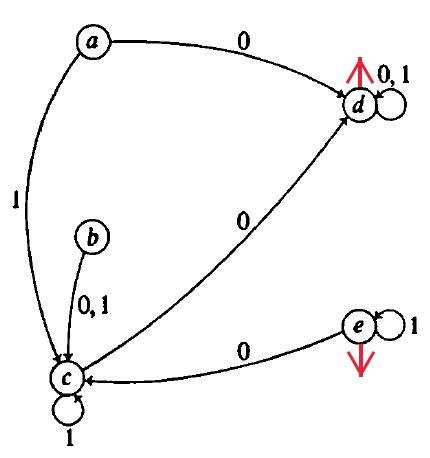
\includegraphics[scale=0.4] {mini-fa} 
	\begin{tikzpicture}[->,>=stealth',shorten >=1pt,auto,node distance=1.5cm, semithick]
	\tikzstyle{every state}=[minimum size=0.1mm]
	\node[state] (a) {$a$};
	\node[state,accepting] (d) [right of=a] {$d$};
	\node[state] (c) [below of=a] {$c$};
	\node[state] (b) [left of=c] {$b$};
	\node[state,accepting] (e) [right of=c] {$e$};
	\path
	(d) edge [loop above] node {$0,1$} (d)
	(c) edge [loop below] node {$1$} (c)
	(e) edge [loop below] node {$1$} (e)
	(a) edge [] node {$0$} (d)
	(a) edge [swap] node {$1$} (c)
	(b) edge [swap] node {$0,1$} (c)
	(e) edge [] node {$0$} (c)
	(c) edge [] node {$0$} (d)
	;
	\end{tikzpicture}
	\caption{Finite state automaton}
	\label{fig:mini-ex2}
\end{figure}

\section{From \cite{Ratnesh95}}

FSM: Finte State Machine

NFSM: Non-deterministic Finite State Machine without $\epsilon-$moves

DFSM: Deterministic Finite State Machine

\begin{definition}[prefix closure of $K$]
	The prefix closure of $K$, denoted $pr(K)\subseteq\Sigma^\ast$, is the language
	\[pr(K):=\{s\in\Sigma^\ast|\exists t\in K:s\le t \}\]
\end{definition}

\begin{example}[Language]\label{ex:language}
	 Consider for example a buffer of capacity one; it has two different states: empty and full. When an \textit{arrival} event occurs in the empty state, then the buffer becomes full; and when a \textit{departure} event occurs in the full state, then the buffer becomes empty. No other state transition can occur in the buffer. Suppose initially the buffer is empty. Then the language of the buffer consists of all possible sequences of the type:
	 $$arrival\cdot departure\cdot arrival\cdot departure \dots,$$
	 where $``\cdot"$ denotes the operation of concatenation.
	 $\hfill\square$
\end{example}

\begin{example}[Generated language]\label{ex:gen_language}
	Consider the buffer of Example \ref{ex:language} Let $a$, $d$ denote the arrival, departure events respectively. Then the generated language of the buffer is $pr((a\cdot d)^\ast)$. Suppose a trace $s\in pr((a\cdot d)^\ast)$ corresponds to completion of a task if and only if its execution results in the empty state of the buffer. Then the marked language of the buffer equals $(a\cdot d)^\ast$.
	$\hfill\square$
\end{example}

\begin{example}[language model]\label{ex:language_model}
	Consider the buffer of Examples \ref{ex:language} and \ref{ex:gen_language} with language	model $[(ad)^\ast,pr((ad)^\ast)]$. The directed graph shown in Figure \ref{fig:DSM} represents a DSM $G:=(X,\Sigma,\alpha,x_0,X_m)$ for the buffer, where $X=\{empty,full\};\Sigma=\{a, d\}; x_0 = empty; X_m = \{empty\};$ and $\alpha(empty, a) = full, \alpha(full, d) = empty$. Note that $\alpha(empty, d)$ and $\alpha(full, a)$ are not defined; hence the transition function is a partial map. (A node in the graph represents a state; a label on a node represents the name of the corresponding state; a directed edge represents a state transition; a label on a directed edge represents the name of the corresponding event; an arrow entering a node represents an initial state; and a circled node represents a marked state.)
	\begin{figure}[htbp]
		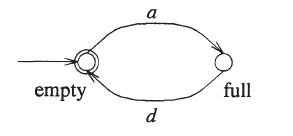
\includegraphics[scale=0.4] {DSM} 
		\caption{Graph representing a DSM}
		\label{fig:DSM}
	\end{figure}
	$\hfill\square$
\end{example}

\begin{example}[Synchronous]
	Consider for example a manufacturing production line consisting
	of a machine (M) and a buffer (B) of capacity one operating in synchrony as shown in Figure \ref{fig:logical-sync}. The event set $\Sigma_1$ of $M$ consists of events $a_1$ representing arrival into the machine, and $d_1$ representing departure from the machine; whereas the event set $\Sigma_2$ of $B$ consists of events $d_1$ representing departure from the machine, and $d_2$ representing departure from buffer. The synchronous composition of two systems is also shown if Figure \ref{fig:logical-sync}.
	\begin{note}
		$d_1$是共享事件,因此,(idle,empty)状态下,$d_1$不能发生, 仅发生 $a_1$事件; (working,empty)状态下,$d_1$在M和B中的转移函数均有定义,因此该共享事件可以发生该共享事件。非共享事件$(a_1,d_2)$在M或B中的转移函数有一个有定义,即可发生。
	\end{note}
	$\hfill\square$
	
	\begin{figure}[htbp]
		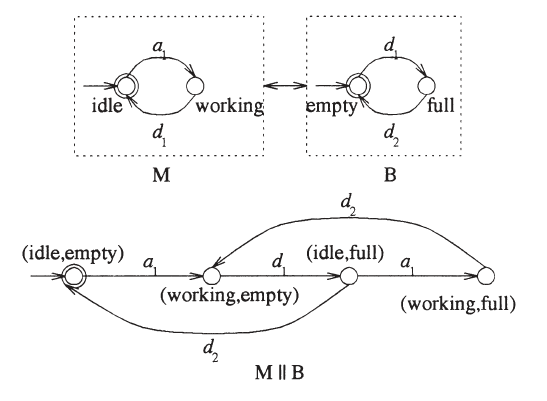
\includegraphics[scale=0.4] {sync} 
		\caption{Diagram illustrating synchronous composition of DFSMs}
		\label{fig:logical-sync}
	\end{figure}
\end{example}

\begin{example}[$\epsilon$-NSM] Consider the $\epsilon$-NSM of Fig. \ref{fig:logical-1model}  Then $\epsilon_G^\ast(1)=\{1,2,3\},\epsilon_G^\ast(2)=\{2,3\},\epsilon_G^\ast(3)=\{3\}.$

so $T(1,\epsilon)=\epsilon_G^\ast(1)=\{1,2,3\}; T(1,a)=\epsilon_G^\ast(T(T(1,\epsilon),a))=\epsilon_G^\ast(T(\{1,2,3\},a)=\epsilon_G^\ast(\{1,3\})=\{1,2,3\}; T(1,ab)=\epsilon_G^\ast(T(\{1,2,3\},b)=\epsilon_G^\ast(\{2\})=\{2,3\}$, etc. $\hfill\square$
	\begin{figure}[htbp]
		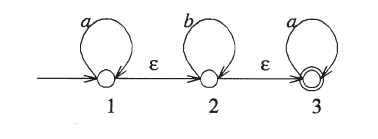
\includegraphics[scale=0.4] {logical-1model} 
		\caption{Diagram illustrating an $\epsilon-NSM$}
		\label{fig:logical-1model}
	\end{figure}
\end{example}


\begin{example}[Completion and reverse]
	Completion and reverse of the DSM of Figure \ref{fig:logical-NFSM-DFSM}(b) are shown
	in Figure \ref{fig:logical-completion-reverse} (a) and \ref{fig:logical-completion-reverse} (b) respectively. The state labels have been changed.
	\begin{figure}[htbp]
		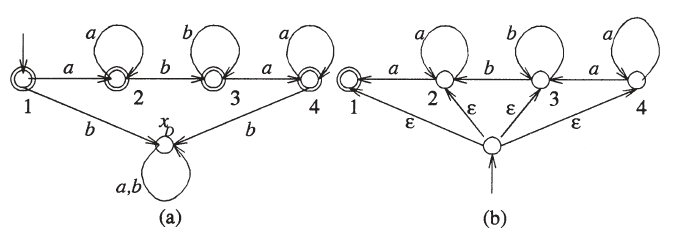
\includegraphics[scale=0.4] {completion-reverse} 
		\caption{Diagram illustrating completion and reverse operations}
		\label{fig:logical-completion-reverse}
	\end{figure}
\end{example}

\begin{theorem}[power set construction]\label{theorem:power_set_cons}
	Let $G:=(X,\Sigma,\alpha,x_0,X_m)$ be a NFSM. Then there exists a language model equivalent DFSM $\mathcal{G}:=(\mathcal{X},\Sigma,\hat{\alpha},\{x_0\},\mathcal{X}_m)$ and $L(\mathcal{G})=L(G)$
\end{theorem}

\begin{proof} Define $\mathcal{X}:=2^X,\mathcal{X}_m:=\{\hat{X}\in\mathcal{X}|\hat{X}\cap X_m\ne \emptyset \}$, and
	\[ \forall \hat{X}\in\mathcal{X},\sigma\in\Sigma:\hat{\alpha}(\hat{X},\sigma):=\bigcup_{x\in\hat{X}}\alpha(x,\sigma) \]
	
	Then is is easily show that $(L_m(\mathcal{G}),L(\mathcal{G}))=(L_m(G),L(G))$
\end{proof}

\begin{example}(NFSM to DFSM)
	Consider the NFSM $G:=(X,\Sigma,\alpha,x_0,X_m)$ shwown in Figure \ref{fig:logical-NFSM-DFSM}(a). The language equivalent DFSM $\mathcal{G}:=(\mathcal{X},\Sigma,\hat{\alpha},\{x_0\},\mathcal{X}_m)$ obtained using the power set construction is shown in Figure \ref{fig:logical-NFSM-DFSM}(b).
	
	Note that $\mathcal{X}=\mathcal{X}_m=\{\{1\},\{1,2,3\},\{2,3\},\{3\} \}$, as $X_m=\{1,3\}$
	
	which has a nonempty intersection with each state in $\mathcal{X}$; 
	\begin{gather*}
	\hat{\alpha}(\{1\},a) = \alpha(1,a) = \{1,2,3\}; \\
	\hat{\alpha}(\{1, 2, 3\}, a) = \alpha(1,a)\cup\alpha(2,a)\cup\alpha(3,a) = \{1, 2, 3\};\\ 
	\hat{\alpha}(\{1, 2, 3\}, b) = \alpha(1, b)\cup\alpha(2, b)\cup\alpha(3, b) = \{2,3\};\\
	etc.
	\end{gather*}

	\begin{figure}[htbp]
		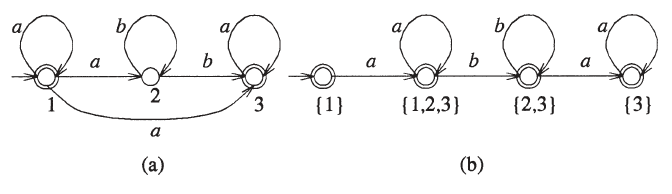
\includegraphics[scale=0.4] {NFSM-DFSM} 
		\caption{Diagram illustrating NFSM to DFSM conversion}
		\label{fig:logical-NFSM-DFSM}
	\end{figure}
\end{example}

\begin{remark}
	It follows from Theorems \ref{theorem:power_set_cons} that if a language model $(K_m, K)$ can be represented as a finite state machine $G$, then there also exists a DFSM $G^\prime$ such that $(L_m(G^\prime), L(G^\prime)) = (K_m, K)$. Thus if we are only concerned with DESs that have finitely many states, then we can assume without loss of generality that they can be represented as DFSMs. We will see below that although the finiteness of states is not needed for most of the analysis, it is needed for developing all the decision algorithms.
	
	However, it should be noted that although DFSMs are useful in developing decision algorithms, it is conceptually easier to obtain a NFSM from the given description of a language. For example, suppose $\Sigma = \{a,b\}$, and suppose we	wish to represent the language with the property that every string in it must contain $aba$ as a substring. A NFSM for the same is shown in Figure \ref{fig:NFSM-DFSM1}(a); corresponding DFSM obtained using the construction outlined in Theorem \ref{theorem:power_set_cons}
	is shown in Figure \ref{fig:NFSM-DFSM1}(b).
\end{remark}

\begin{figure}[htbp]
	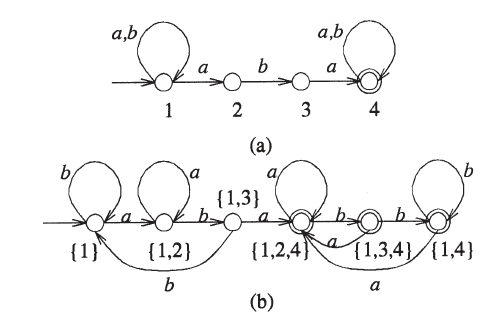
\includegraphics[scale=0.4] {NFSM-DFSM1} 
	\caption{NFSM accepting strings with aba as a substring, and corresponding DFSM}
	\label{fig:NFSM-DFSM1}
\end{figure}

\subsection{Myhill-Nerode Characterization}

\begin{definition}[equivalence relation$(R_K)$]
	Given a language $K\subseteq \Sigma^\ast$, it induces an equivalence relation, denoted $R_K$, on $\Sigma^\ast$:
	\[ \forall s,t\in\Sigma^\ast: s\cong t(R_K)\Leftrightarrow [K\setminus\{s\}=K\setminus\{t\}] \]
	For each $s\in\Sigma^\ast,[s]R_K\subseteq\Sigma^\ast$ is used to denote the equivalence class containing the string $s$.
\end{definition}

\begin{definition}[equivalence relation$(R_G)$]
	Given a DFSM $G:=(X,\Sigma,\alpha,x_0,X_m)$, it induces an equivalence relation, denoted $R_G$, on $\Sigma^\ast$:
	\[ \forall s,t\in\Sigma^\ast: s\cong t(R_G)\Leftrightarrow [\alpha(x_0,s)=\alpha(x_0,t)]\lor[\alpha(x_0,s)=\alpha(x_0,t) \text{ undefined}] \]
	For each $s\in\Sigma^\ast,[s]R_G\subseteq\Sigma^\ast$ is used to denote the equivalence class containing the string $s$.
\end{definition}

\begin{note}
	Note the $R_G$, the \textit{index} of $R_G$, i.e., the number of equivalence classes of $R_G$, is one more than the number of states in $G$, $|R_G|=|G|+1$. (The set of all strings that do not
	belong to $L(G)$ belong to a single equivalence class of $R_G$.) 
\end{note}

It can be easily seen that the equivalence relation $R_G$ refines the equivalence relations $R_{L_m(G)}$ and $R_{L(G)}$. In other words,
\[ \forall s,t\in\Sigma^\ast : s\cong t(R_G)\Rightarrow [s\cong t(R_{L_m(G)})]\land [s\cong t(R_{L(G)})] \]

An equivalence relation $R$ on $\Sigma^\ast$ is said to be \textit{right invariant (with respect to concatenation)} if
\[ \forall s,t\in\Sigma^\ast : s\cong t(R) \Rightarrow su\cong tu(R) \]

It is easy to verify that $R_K$ as well as $R_G$ defined above are right invariant.The following proposition is due to Myhill and Nerode:

\begin{theorem}[Myhill and Nerode]\label{theorem:MyhillNerode}
	Let $K\subseteq\Sigma^\ast$ be a language. Then the following are equivalent:
	\begin{enumerate}[1. ]
		\item $K$ is regular.
		\item $K$ can be written as union of some of the equivalence classes of a right invariant equivalence relation of finite index.
		\item $R_K$ is of finite index.
	\end{enumerate}
\end{theorem}

\begin{proof}
	$(1)\Rightarrow (2)$: Suppose $K$ is regular. Then there exists a DFSM $G$ such that $L_m(G) = K$. Then clearly $K$ can be written as union of the following equivalence classes of $R_G$:
	\[\{[s](R_G)|s\in K \}\]
	
	This proves the first assertion implies the second assertion, as $R_G$ is right invariant.
	
	$(2)\Rightarrow (3)$: Let R be a right invariant equivalence relation of finite index such that $K$ can be written as union of some of the equivalence classes of $R$. In order to show that $R_K$ is of finite index it suffices to show that $R$ refines $R_K$. Pick $s,t\in\Sigma^\ast$  such that $s\cong t(R)$. Since $R$ is right invariant, for any $u\in\Sigma^\ast,su\cong tu(R)$. Since $K$ equals union of some of the equivalence classes of $R$, this implies $su\in K$ if and only if $tu\in K$. In other words, $s\cong t(R_K)$, which proves that the second assertion implies the third assertion.
	
	$(3)\Rightarrow (1)$: Finally, suppose $R_K$ is of finite index. Define a DFSM $G:=(\hat{X},\Sigma,\hat{\alpha},\hat{x}_0,\hat{X}_m)$ as follows: $\hat{X}:=\{[s](R_K)|s\in\Sigma^\ast\}; x_0 :=[\epsilon](R_K); \hat{X}_m=\{[s](R_K)|s\in K \}$;
	and
	\[ \forall [s](R_k)\in\hat{X},\sigma\in\Sigma:\hat{\alpha}([s](R_K),\sigma):=[s\sigma](R_K) \]
	
	Then it is readily verified that for each $s\in\Sigma^\ast,\hat{\alpha}(\hat{x}_0,s)=[s](R_K)$. Hence
	from definition of marked language we obtain that $s\in L_m(G)$ if and only if $\hat{\alpha}(\hat{x}_0,s) = [s](R_K) \in X_m$, i.e., if and only if $s\in K$. Thus $L_m(G) = K$. Since $\hat{G}$ is a DFSM (as $R_K$ is of finite index), this implies that $K$ is regular; so the third assertion implies the first assertion. $\hfill\square$
\end{proof}

The construction of the DFSM G in the proof of Theorem \ref{theorem:MyhillNerode} is known as the Myhill-Nerode construction. The following example illustrates such a construction.

\begin{example}[equivalence classes]
	Consider for example the marked language $K_m = (ad)^\ast$ of
	the buffer of capacity one of Example \ref{ex:gen_language}. 
	Then the generated language of the buffer is $pr((a\cdot d)^\ast)=pr(K_m)$. Suppose a trace $s\in pr((a\cdot d)^\ast)$ corresponds to completion of a task if and only if its execution results in the empty state of the buffer. Then the marked language of the buffer equals $(a\cdot d)^\ast$.
	
	Clearly, $K_m$ is a regular language.
	Hence it follows from Theorem \ref{theorem:MyhillNerode} that $R_{K_m}$ is of finite index. It can be easily verified that
	\begin{gather*}
		[\epsilon](R_{K_m})=(ad)^\ast=K_m\\
		[a](R_{K_m})=(ad)^\ast a=pr(K_m)-K_m\\
		[d](R_{K_m})=\{a,d\}^\ast-pr(K_m)
	\end{gather*}
	and these are the only equivalence classes of $R_{K_m}$
	
	Hence Myhill-Nerode construction yields the DFSM $G:=(\hat{X},\Sigma,\hat{\alpha},\hat{x}_0,\hat{X}_m)$, while\\ 
	$\hat{X}=\{[\epsilon](R_{K_m}),[a](R_{K_m}),[d](R_{K_m}) \}$;
	$\hat{x}_0=[\epsilon](R_{K_m}); X_m=\{[\epsilon](R_{K_m}) \}$;\\
	and
	\begin{align*}
		\hat{\alpha}([\epsilon](R_{K_m}),a)&=[a](R_{K_m});\\
		\hat{\alpha}([\epsilon](R_{K_m}),d)&=[d](R_{K_m});\\
		\hat{\alpha}([a](R_{K_m}),a)&=[aa](R_{K_m})=[d](R_{K_m});\\
		\hat{\alpha}([a](R_{K_m}),d)&=[ad](R_{K_m})=[\epsilon](R_{K_m});\\
		\hat{\alpha}([d](R_{K_m}),a)&=[da](R_{K_m})=[d](R_{K_m});\\
		\hat{\alpha}([d](R_{K_m}),d)&=[dd](R_{K_m})=[d](R_{K_m});
	\end{align*}
	
	See figure \ref{fig:equiv}, State e: empty,$[\epsilon](R_{K_m})$;
	State f: full,$[a](R_{K_m})$;  State t: dump/trap,$[d](R_{K_m})$.
	
	\begin{figure}[htbp]
      \centering
	  \subfigure[buffer model]
	  {
	  	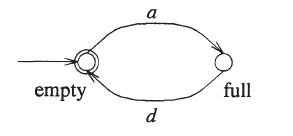
\includegraphics[scale=0.4] {DSM}
	  }
      \hspace{2cm} % 如果并列,用\\换行即可
      \subfigure[equivalence classes]
      {
		  \begin{tikzpicture}[->,>=stealth',shorten >=1pt,auto,node distance=2cm, semithick]
		  \tikzstyle{every state}=[minimum size=0.1mm]
		  \node[state]         (t) {t};
		  \node[initial,state,accepting] (e) [above left of=t] {e};
		  \node[state]         (f) [above right of=t] {f};
		  \path
		  (e) edge [bend left]  node {$a$} (f)
		      edge [swap] node {$d$} (t)
		  (f) edge [bend left]  node {$d$} (e)
		      edge [] node {$a$} (t)
		  ;
		  \end{tikzpicture}
		  (states e:empty,f:full,t:dump/trap) 
      }
	  \caption{equivalence classes}
	  \label{fig:equiv}
	\end{figure}
	$\hfill\square$
\end{example}

\begin{remark}
	Given a regular language K, there always exists a DFSM $G$ such
	that $L_m(G) = K$. Hence there exists a minimal such DFSM (one with a minimal number of states). Let $G^\prime$ be the DFSM obtained by removing the state $[s](R_K)$ form $\hat{G}$ (and all transitions leading into/out of it), where $\hat{G}$ is the DFSM in the proof of Theorem \ref{theorem:MyhillNerode} and $s\in \Sigma^\ast$ is such that $s\notin pr(K)$.Then it is easy to see that $L_m(G^\prime) = K$. In fact $G^\prime$ is a minimal DFSM with marked language $K$. In order to see this first note that the number of states in $\hat{G}$ is $|R_K|$, the index of $R_K$. Since $G^\prime$ is obtained by removing a single state from $\hat{G}$, the number of states in $G^\prime$ equals $|R_K|-1$. Let $G$ be any DFSM with $L_m(G) = K$. Then as noted above number of states in $G$ equals $|R_G|-1$. Also,as noted above, $R_G$ refines $R_{L_m(G)} = R_K$, which implies that $|R_K|\le |R_G|$. Thus $|R_K| - 1\le |R_G| - 1$, which proves that $G^\prime$ is a minimal DFSM with marked language $K$.
\end{remark}

\subsection{Minimization}

\begin{theorem}[Minimal $K$] \label{theorem:Minimal}
	Suppose $K\subseteq \Sigma^\ast$ is a regular language. Then a trim DFSM $G:=(X,\Sigma,\alpha,x_0,X_m)$ with marked language $K$ is mininmal if and only if
	$$\forall x,x^\prime\in X,s\in \Sigma^\ast :(\alpha(x,s),\alpha(x^\prime,s))\in X_m\times X_m\Rightarrow x=x^\prime .$$
\end{theorem}

Suppose $K\subseteq \Sigma^\ast$ is regular. Let $G:=(X,\Sigma,\alpha,x_0,X_m)$ be a trim DSFSM such that $L_m(G)=K$. We are interested in obtaining a minimal DFSM with marked language $K$ by combining some of the ``language equivalent" states of $G$. Note that if $K = \Sigma^\ast$, then it can be accepted by a minimal DFSM having a single state. Hence we assume without loss of generality that $K\ne\Sigma^\ast$.

DFSM $G:=(X,\Sigma,\alpha,x_0,X_m)$ induces an equivalence relation on $X$ defined as:
\[ \forall x,x^\prime\in X:x\cong x^\prime \Leftrightarrow [\forall s\in\Sigma^\ast:\alpha(x,s)\in X_m\Leftrightarrow\alpha(x^\prime,s)\in X_m] \]

Using this equivalence relation we define a language equivalent DFSM $\hat{G}:=(\hat{X},\Sigma,\hat{\alpha},\hat{x}_0,\hat{X}_m)$, where $\hat{X}:=\{[x]|x\in X\},\hat{x}_0:=[x_0],\hat{X}_m:=\{[x]|x\in X_m\}$, and
\[
\forall [x]\in\hat{X},\sigma\in\Sigma:\hat{\alpha}([x],\sigma):=\left\{ 
\begin{aligned}
\left[\alpha(x,\sigma)\right]  &\text{   if $\alpha(x,\sigma)$ defined}\\ 
\text{undefined} &\text{    otherwise}\\
\end{aligned} 
\right. 
\]

Using the fact that $G$ is trim, it is readily verified that $\hat{G}$ is well defined, and $(L_m(\hat{G}),L(\hat{G}))=(L_m(G),L(G))=(K,pr(K))$. Moreover, it follows from Theorem \ref{theorem:Minimal} that $\hat{G}$ is a minimal state machine with marked language $K$.

An algorithm for efficiently identifying the equivalence classes $\{[x]|x\in X\}$ is presented next. Note that each state pair $(x,x^\prime)\in (X_m\times X_m)\cup [(X-X_m)\times (X-X_m)]$ is a possible pair of equivalent states. 

First consider $\bar{G}:=(\bar{X},\Sigma,\bar{\alpha},x_0,X_m)$, the completion of $G$. Then since $K\ne\Sigma^\ast,X_m\ne\bar{X}=X\cup\{x_D\}$, while $X_D$ is the ``dump" state. This implies $\bar{X}-X_m\ne\emptyset$.

\begin{note}
	Note that if $K = \Sigma^\ast$, then it can be accepted by a minimal DFSM having a single state.
\end{note}

\begin{figure}[htbp]
	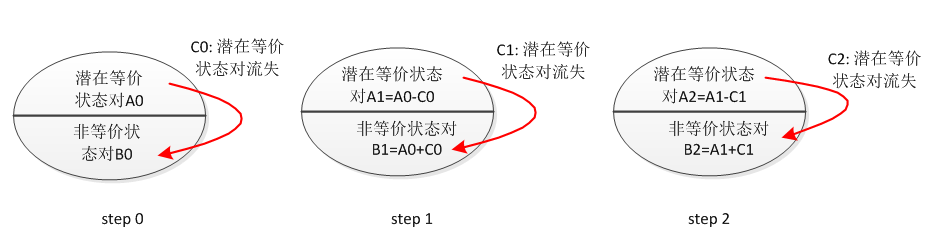
\includegraphics[scale=0.4] {algo-minimize} 
	\caption{Diagram illustrating algorithm minimize}
	\label{fig:algo-minimize}
\end{figure}

\begin{algorithm}  
	\caption{The algorithm for a minimal DFSM, see Figure \ref{fig:algo-minimize}}  
	\begin{algorithmic}[1] %每行显示行号  
		\Require $G=(\bar{X},\Sigma,\alpha,\_,X_m)$  
		\Ensure The equivalence classes of $X$ 
		
		A: \{潜在等价状态对\}; B: \{非等价状态对\}; C: \{本次迭代流失的潜等价状态对\}
		
		\State Initiation step:
		
		$A_0 := [X_m\times X_m]\cup [(\bar{X}-X_m)\times(\bar{X}-X_m)]=\{\text{(final状态对)}\cup \text{(非final状态对)} \} = \{\text{潜在的等价状态对}\}$; 
		
		$B_0 := [\bar{X}\times\bar{X}-A_0] = \{\text{(全体状态对)}-A_0 \} = \{\text{(final状态,非final状态)} \} = \{\text{非等价状态对}\} = \{\text{非$A_0$状态对}\}$; 
		
		$k:=0$.
		
		\State Iteration step:
		\begin{align*}
			C_k &:= \{(x,x^\prime)\in A_k | \exists\sigma\in\Sigma \text{ s.t. } (\alpha(x,\sigma),\alpha(x^\prime,\sigma))\in B_k \} \\
			&=\{\text{$A_0$中两大类中的(状态对)存在字母$\sigma$进入$B_0$类)} \} \\
			&= \{ \text{潜在状态对 $\to$ 非等价状态对} \}\\
			A_{k+1} &:= A_k - C_k \\
			B_{k+1} &:= B_k\cup C_k =[\bar{X}\times \bar{X}] - A_{k+1}\\
			&=\{\text{非$A_{k+1}$状态对}\}
		\end{align*}
		
		\State Termination step:
		
		if $A_{k+1}=A_k$, then stop; else, $k := k+1$, and goto step 2.
	\end{algorithmic}
    \label{alg:minimal}   
\end{algorithm}

It can be verified that after termination, each state pair in $A_k$ is an equivalent pair of states. Finally, the minimal state machine $G$ is obtained by combining each state pair in $A_k$ as described above, and removing the equivalence class of the dump state.

Algorithm \ref{alg:minimal} terminates in $O(m^2)$ steps, where $m$ is the number of states in $G$.

\begin{example}
	Consider the complete DFSM of Figure \ref{fig:complete}. Then $X_m=\{1,2,3,4 \}$ and $X=\{1,2,3,4,x_D \}$. Algorithm \ref{alg:minimal} can be  applied to minimize the DFSM as follows:
	\begin{align*}
		A_0 &=[X_m\times X_m]\cup\{(x_D\times x_D)\};\\
		&=\{(1,1),(2,2),(3,3),(4,4),(1,2),(2,1),(1,3),(3,1),(1,4),(4,1),(2,3),(3,2),(2,4),(4,2),(3,4),(4,3) \} \cup\{(x_D,x_D) \}\\
		&=\{(1,1),(2,2),(3,3),(4,4) \}\cup\{(1,2),(1,3),(1,4),(2,3),(2,4),(3,4) \}\cup
		\{(2,1),(3,1),(4,1),(3,2),(4,2),(4,3)\}\cup\{x_D,x_D\}\\
		&= \{\text{潜在的等价状态对}\} \\
		B_0 &=[X\times X]-A_0\\
		&=\{(1,x_D),(x_D,1),(2,x_D),(x_D,2),(3,x_D),(x_D,3),(4,x_D),(x_D,4) \}\\
		&=\{(1,x_D),(2,x_D),(3,x_D),(4,x_D) \} \cup \{(x_D,1),(x_D,2),(x_D,3),(x_D,4) \}\\
		&= \{\text{非等价状态对}\} = \{\text{非$A_0$状态对}\}\\
		C_0 &= \{(1,2),(2,1),(1,3),(3,1),(2,4),(4,2),(3,4),(4,3)\}\\
		&=\{(1,2),(1,3),(2,4),(3,4) \}\cup\{(2,1),(3,1),(4,2),(4,3) \}\\
		&= \{ \text{潜在状态对$(A_0) \to (B_0)$非等价状态对} \}\\
		A_1 &= A_0-C_0\\
		&=\{(1,1),(2,2),(3,3),(4,4) \}\cup\{(1,4),(2,3) \}\cup
		\{(4,1),(3,2) \}\cup\{x_D,x_D\}\\
		B_1 &= [X\times X]-A_1\\
		&= \{\text{非$A_1$状态对}\}\\
		C_1 &= \{ \text{潜在状态对($A_1) \to (B_1)$非等价状态对} \}\\
		&= \{(1,4),(4,1),(2,3),(3,2)\}\\
		A_2 &= A_1-C_1\\
		&= \{(1,1),(2,2),(3,3),(4,4),(x_D,x_D)\}\\
		B_2 &=[X\times X] - A_2
	\end{align*}
    Clearly, all the state pairs in $A_2$ are equivalent pairs, i.e. $C_2 = \emptyset$: hence the algorithm terminates. Thus the minimal DFSM is the DFSM of Figure \ref{fig:complete}, which does not contain the dump state.
	\begin{figure}[htbp]
		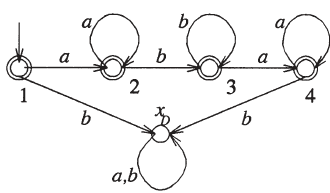
\includegraphics[scale=0.4] {complete} 
		\caption{the minimal DFSM is not contain the dump state}
		\label{fig:complete}
	\end{figure}
\end{example}

\section{From wiki -- Partition of a set}

From \url{https://en.wikipedia.org/wiki/Partition_of_a_set}.

\begin{definition}[a partition of a set] 
	A partition of a set $X$ is a set of nonempty subsets of $X$ such that every element $x$ in $X$ is in exactly one of these subsets (i.e., $X$ is a disjoint union of the subsets).
	Equivalently, a family of sets $P$ is a partition of $X$ if and only if all of the following conditions hold:
	\begin{itemize}
		\item The family $P$ does not contain the empty set (that is $\emptyset \notin P)$.
		\item The union of the sets in $P$ is equal to $X$ (that is $\bigcup _{A\in P}A = X)$ . The sets in $P$ are said to \textbf{cover} $X$.
		\item The intersection of any two distinct sets in $P$ is empty (that is $(\forall A,B\in P)\;A\neq B\implies A\cap B=\emptyset)$. The elements of $P$ are said to be pairwise disjoint.
	\end{itemize}
	
	The sets in P are called the \textit{blocks, parts} or \textit{cells} of the partition.
	
	The rank of $P$ is $|X| − |P|$, if $X$ is finite.
\end{definition}

\begin{example}[a partition of a set]
	(From \url{https://en.wikipedia.org/wiki/Partition_of_a_set})
	\begin{itemize}
		\item The empty set $\emptyset$ has exactly one partition,namely $\emptyset$.
		\item For any nonempty set $X, P = \{X\}$ is a partition of $X$, called the trivial partition.
		\subitem Particularly, every singleton set $\{x\}$ has exactly one partition, namely $\{ \{x\} \}$.
		\item For any non-empty proper subset $A$ of a set $U$, the set $A$ together with its complement form a partition of $U$, namely, $\{A, U \setminus A \}$.
		\item The set $\{ 1, 2, 3 \}$ has these five partitions (one partition per item):
		\begin{itemize}
			\item $\{ \{1\}, \{2\}, \{3\} \}$, sometimes written $1|2|3$.
			\item $\{ \{1, 2\}, \{3\} \}$, or $12|3$.
			\item $\{ \{1, 3\}, \{2\} \}$, or $13|2$.
			\item $\{ \{1\}, \{2, 3\} \}$, or $1|23$.
			\item $\{ \{1, 2, 3\} \}$, or $123$ (in contexts where there will be no confusion with the number).
		\end{itemize}
		\item The following are not partitions of $\{ 1, 2, 3 \}$:
		\begin{itemize}
			\item \{ \{\}, \{1, 3\}, \{2\} \} is not a partition (of any set) because one of its elements is the empty set.
			\item $\{ \{1, 2\}, \{2, 3\} \}$ is not a partition (of any set) because the element $2$ is contained in more than one block.
			\item $\{ \{1\}, \{2\} \}$ is not a partition of $\{1, 2, 3\}$ because none of its blocks contains $3$; however, it is a partition of $\{1, 2\}$.
		\end{itemize}
	\end{itemize}
\end{example}

\begin{definition}[Partitions and equivalence relations]
	For any equivalence relation on a set $X$, the set of its equivalence classes is a partition of $X$. Conversely, from any partition $P$ of $X$, we can define an equivalence relation on $X$ by setting $x\equiv y$ precisely when $x$ and $y$ are in the same part in $P$. Thus the notions of equivalence relation and partition are essentially equivalent.
	
	The axiom of choice guarantees for any partition of a set $X$ the existence of a subset of $X$ containing exactly one element from each part of the partition. This implies that given an equivalence relation on a set one can select a canonical representative element from every equivalence class.
\end{definition}

\begin{definition}[Refinement of partitions]
	A partition $\alpha$ of a set $X$ is a refinement of a partition $\rho$ of $X$—and we say that $\alpha$ is finer than $\rho$ and that $\rho$ is coarser than $\alpha$—if every element of $\alpha$ is a subset of some element of $\rho$. Informally, this means that $\alpha$ is a further fragmentation of $\rho$. In that case, it is written that $\alpha\le\rho$.
	
	This finer-than relation on the set of partitions of $X$ is a partial order (so the notation $``\le"$ is appropriate). Each set of elements has a least upper bound and a greatest lower bound, so that it forms a lattice, and more specifically (for partitions of a finite set) it is a geometric lattice. The partition lattice of a 4-element set has 15 elements and is depicted in the Hasse diagram on the Fig \ref{fig:Hasse}.
	
	Based on the cryptomorphism between geometric lattices and matroids, this lattice of partitions of a finite set corresponds to a matroid in which the base set of the matroid consists of the atoms of the lattice, namely, the partitions with $n-2$ singleton sets and one two-element set. These atomic partitions correspond one-for-one with the edges of a complete graph. The matroid closure of a set of atomic partitions is the finest common coarsening of them all; in graph-theoretic terms, it is the partition of the vertices of the complete graph into the connected components of the subgraph formed by the given set of edges. In this way, the lattice of partitions corresponds to the lattice of flats of the graphic matroid of the complete graph.
	
	Another example illustrates the refining of partitions from the perspective of equivalence relations. If D is the set of cards in a standard 52-card deck, the same-color-as relation on D – which can be denoted ~C – has two equivalence classes: the sets {red cards} and {black cards}. The 2-part partition corresponding to ~C has a refinement that yields the same-suit-as relation ~S, which has the four equivalence classes {spades}, {diamonds}, {hearts}, and {clubs}.
	
	\begin{figure}[htbp]
		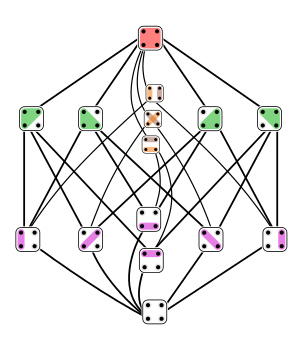
\includegraphics[scale=0.8]{Hasse.png}
		\caption{Partitions of a 4-set ordered by refinement}
		\label{fig:Hasse}
	\end{figure}
\end{definition}

\section{From \cite{Kenneth2012}}

\begin{definition}[等价关系]
	定义在集合$A$上的关系叫做等价关系,如果它是自反的、对称的和传递的。
\end{definition}

\begin{definition}[等价元素]
	如果两个元素$a$和$b$由于等价关系而相关联,则称它们是等价的。记法$a\sim b$通常用来表示对于某个特定的等价关系来说,$a$和$b$是等价的元素。
\end{definition}

\begin{note}
	在等价关系中,若两个元素有关系,就可以说它们是等价的。为了使等价元素的概念有意义,每个元素都应该等价于它自身,因为对于等价关系来说,自反性是一定成立的。在等价关系中,说$a$和$b$是相互关联也是正确的(而不仅是$a$关联于$b$),因为如果$a$关联于$b$, 右对称性, $b$也关联于$a$。
	
	此外,因为等价关系是传递的,所以如果$a$和$b$等价且$b$和$c$等价,则可得出$a$和$c$也是等价的。
\end{note}

\begin{example}
	设$R$是定义在整数集上的关系,满足$aRb$当且仅当$a=b$或$a=-b$。可以证明$R$是自反的,对称的和传递的。因此$R$是等价关系。
\end{example}

\begin{example}[模$m$同余]
	设$m$是大于1的整数。证明以下关系是定义在整数集上的等价关系。
	\[R=\{(a,b)|a\equiv b\pmod{m}\} \]
\end{example}

\begin{proof}
	$a\equiv b\pmod{m}$, 当且仅当$m$整除$a-b$。 注意$a-a=0$能被$m$整除,因为$0=0\cdot m$。因此$a\equiv a\pmod{m}$, 从而模$m$同余关系是自反的。
	
	假设$a\equiv b\pmod{m}$, 那么$a-b$能被$m$整除,即$a-b=km$, 其中$k$是整数。从而$b-a=(-k)m$, 即$b\equiv a\pmod{m}$, 因此模$m$同余关系是对称的。
	
	下面假设$a\equiv b\pmod{m}$和$b\equiv c\pmod{m}$, 那么$m$整除$a-b$和$b-c$。因此存在整数$k$和$l$, 使得$a-b=km$和$b-c=lm$, $\implies a-c=(a-b)+(b-c)=km+lm=(k+l)m$。于是$a\equiv c\pmod{m}$, 从而模$m$同余关系是传递的。
	
	综上所述,模$m$同余关系是等价的。
\end{proof}

\begin{example}
	设$R$是定义在英文字母组成的字符串的集合上的关系,满足$aRb$当且仅当$l(a)=l(b)$, 其中$l(x)$是字符串$x$的长度。证明$R$是等价关系。
\end{example}

\begin{proof}
	因为$l(a)=l(a)$, 所以只要$a$是一个字符串,就有$aRa$, 故$R$是自反的。其次,假设$aRb$, 即$l(a)=l(b)$, 那么有$bRa$, 因为$l(b)=l(a)$, 所以$R$是对称的。最后,假设$aRb$且$bRc$, 那么有$l(a)=l(b),l(b)=l(c)\implies l(a)=l(c)$, 即$aRc$, 从而$R$是传递的。由于$R$是自反的,对称的和传递的,所以$R$是等价关系。
\end{proof}

\begin{example}\label{ex:eqstr}
	设$n$是正整数,$S$是字符串集合。假定$R_n$是$S$上的关系,$sR_n t$当且仅当$s=t$或者$s$和$t$都至少含有$n$个字符,且$s$和$t$的前$n$个字符相同。就是说,少于$n$个字符的字符串只于它自身的$R_n$相关;一个至少含有$n$个字符的字符串$s$与字符串$t$相关当且仅当$t$也含有至少$n$个字符且$t$以$s$最前面的$n$个字符开始。例如,设$n=3$, $S$是所有位串的集合,$sR_3t$当$s=t$或者$s$和$t$均为长度至少为3的位串,且前3位相同。例如,$01R_3 01$, $00111R_3 001101$,但是$(01,010)\notin R_3, (0101,01110)\notin R_3$
	
	证明:对所有的字符串集$S$和所有的正整数$n$, $R_n$是定义在$S$上的等价关系。
\end{example}

\begin{proof}
	
	设$s$是$S$中的一个字符串,由于$s=s$, 可得$sR_ns$, 所以$R_n$关系是自反的。
	
	如果$sR_nt$, 那么或者$s=t$或者$s$和$t$都至少含有$n$个字符,且以相同的$n$个字符开始。这意味着$tR_ns$成立。所以$R_n$是对称的。
	
	现在假设$sR_nt$且$tR_nu$。 则有$s=t$或者$s$和$t$都至少含有$n$个字符,且以相同的$n$个字符开始。还有$t=u$或者$t$和$u$都至少含有$n$个字符,且以相同的$n$个字符开始。 由此可以推出$s=u$或者$s$和$u$都至少含有$n$个字符,且以相同的$n$个字符开始(因为在这种情形下,我们知道$s,t$和$u$都至少含有$n$个字符,且$s$和$u$都与$t$一样以相同的$n$个字符开始)。所以$R_n$是传递的。
	
	综上所述,模$R_n$是一个等价关系。
\end{proof}

\begin{definition}[等价类]
	设$R$是定义在集合$A$上的等价关系。与$A$中的一个元素$a$有关系的所有元素的集合叫做$a$的等价类。$A$的关于$R$的等价类记作$[a]_R$。当只考虑一个关系时,我们将省去下标$R$并把这个等价类写作$[a]$。
	
	换句话说,如果$R$是定义在集合$A$上的等价关系,则元素$a$的等价类是
	\[ [a]_R = \{s|(a,s)\in R \}\]
	如果$b\in [a]_R,b$叫做这个等价类的\textbf{代表元}。一个等价类的任何元素都可以作为这个类的代表元。也就是说,选择特定元素作为一个类的代表元没有特殊要求。 
\end{definition}

\begin{example}
	设$R$是定义在整数集上的关系,满足$aRb$当且仅当$a=b$或$a=-b$。可以证明$R$是自反的,对称的和传递的。因此$R$是等价关系。
	
	在这个等价关系中,一个整数对应于它自身和它的相反数数。从而一个整数的等价类是:$[a]=\{a,-a\}$。这个集合包含两个不同的整数,除非$a=0$。例如, $[7]=\{7,-7\},[-5]=\{-5,5\},[0]=\{0\}$。
\end{example}

\begin{example}
	对于模$4$同余关系,0和1的等价类是什么?
	
	0的等价类包含使得$a\equiv 0\pmod{4}$的所有整数$a$。这个类中的整数是能被4整除的那些整数。因此,对于这个关系,0的等价类是
	\[ [0]=\{\cdots,-8,-4,0,4,8,\cdots \}\]
	1的等价类包含使得$a\equiv 1\pmod{4}$的所有整数$a$。这个类中的整数是当被4除时余数为1的那些整数。因此,对于这个关系,1的等价类是
	\[ [1]=\{\cdots,-7,-3,1,5,9,\cdots \}\]
	
	用正整数$m$代替4, 很容易推广到模m同余关系的等价类--模m的同余类。整数$a$模$m$的同余类记作$[a]_m$, 满足
	\[ [a]_m=\{\cdots,a-2m,a-m,a,a+m,a+2m,\cdots \}\] 
	例如,
	\begin{align*}
		[0]_4 &=\{\cdots,-8,-4,0,4,8,\cdots \} \\
		[1]_4 &=\{\cdots,-7,-3,1,5,9,\cdots \} 
	\end{align*}
		
\end{example}

\begin{example}
	对于例\ref{ex:eqstr}中所有位串集合上的等价关系$R_3$, 串$0111$的等价类是什么?
	等价于$0111$的是以$011$开始,至少含有3位的位串:
	\[[011]_{R_3}=\{011,0110,0111,01100,01101,0111111,\cdots\}\]
\end{example}

\begin{theorem} \label{theorem:eqPro}
	设$R$是定义在集合$A$上的等价关系,下面的关于集合$A$中$a,b$两个元素的命题是等价的。
	\begin{enumerate}[(i) ]
		\item $aRb$
		\item $[a]=[b]$
		\item $[a]\cap [b]\ne\emptyset$
	\end{enumerate}
\end{theorem}

\begin{proof}
	首先证明(i)推出(ii)。
	
	假设$aRb$,我们将通过$[a]\subseteq [b]$和$[b]\supseteq [a]$来证明$[a]=[b]$。
	
	假设$c\in [a]$, 那么$aRc$。因为$aRb$是对称的,所以$bRa$。又由于$R$是传递的以及$bRa$和$aRc$, 就得到$bRc$, 所以$c\in [b]$。这就证明了$[a]\subseteq [b]$。 类似地,可证明$[a]\supseteq [b]$。
	
	其次我们将证明(ii)推出(iii)。假设$[a]=[b]$, 这就证明了$[a]\cap [b]\ne\emptyset$, 因为$[a]$是非空的(由$R$的自反性$a\in [a]$)。
	
	下面证明(iii)推出(i)。假设$[a]\cap [b]\ne\emptyset$, 那么存在元素$c$满足$c\in [a]$且$c\in [b]$。换句话说, $aRc$且$bRc$。由对称性, 有$cRb$。再根据传递性,由$aRc$和$cRb$,就有$aRb$。
	
	因为$(i)\implies (ii),(ii)\implies (iii),(iii)\implies (i)$, 所以三个命题是等价的。
\end{proof}

现在我们将说明一个等价关系怎样划分一个集合。设$R$是定义在集合$A$上的的等价关系,$R$的所有等价类的并集就是集合$A$, 因为$A$的每个元素$a$都在它自己的等价类,即$[a]_R$中。换句话说,
\[ \bigcup_{a\in A}[a]_R = A \]
此外,有定理\ref{theorem:eqPro},这些等价类或者是相等的或者是不相交的的,因此当$[a]_R\ne[b]_R$时,
\[ [a]_R\cap [b]_R = \emptyset\]

这两个结论证明了等价类构成$A$的划分, 因为它们将$A$分成不相交的子集。更确切的说,集合$S$的\textbf{划分}是$S$的不相交的非空的子集构成的集合,且它们的并集就是$S$。换句话说,一簇子集$A_i,i\in I$, (其中$I$是下标的集合)构成$S$的划分,当且仅当
\begin{align*}
A_i &\ne \emptyset  &i\in I \\
A_i\cap A_j &=\emptyset  &i\ne j\\
\bigcup_{i\in I}A_i &= S  &
\end{align*}

\begin{figure}[htbp]
	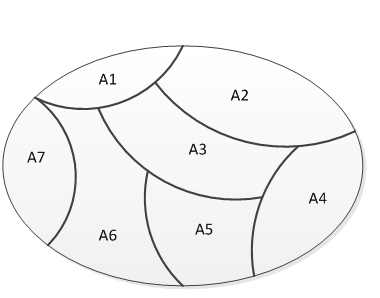
\includegraphics[scale=.4]{partition}
	\caption{Partition of set}
	\label{fig:partition}
\end{figure}

\begin{example}
	假设$S=\{1,2,3,4,5,6\}$, 一簇集合$A_1=\{1,2,3\},A_2=\{4,5\},A_3=\{6\}$构成$S$的一个划分,因为这些集合是不相交的,且它们的并集是$S$。
\end{example}

\begin{theorem}
	设$R$是定义在集合$S$上的等价关系。那么$R$的等价类构成$S$的划分。反过来,给定集合$S$的划分$\{A_i|i\in I\}$, 则存在一个等价关系$R$,它以集合$A_i(i\in I)$作为它的等价类。
\end{theorem}

\begin{example}
	假设$S=\{1,2,3,4,5,6\}$, 一簇集合$A_1=\{1,2,3\},A_2=\{4,5\},A_3=\{6\}$构成$S$的一个划分,因为这些集合是不相交的,且它们的并集是$S$。
	列出这个划分所产生的等价关系$R$中的有序对。
\end{example}

\begin{solution}
	划分中的子集是$R$的等价类。有序对$(a,b)\in R$, 当且仅当$a$和$b$在划分的同一个子集中。
	
	由于$A_1=\{1,2,3\}$是一个等价类,因此有序对$(1,1),(1,2),(1,3),(2,1),(2,2),(2,3),(3,1),(3,2),(3,3)$属于$R$。
	
	由于$A_2=\{4,5\}$是一个等价类,因此有序对$(4,4),(4,5),(5,4),(5,5)$也属于$R$。
	
	由于$A_3=\{6\}$是一个等价类,因此有序对$(6,6)$也属于$R$。
\end{solution}

\begin{example}
    模m同余关系的等价类--模m的同余类。整数$a$模$m$的同余类记作$[a]_m$, 满足
	\[ [a]_m=\{\cdots,a-2m,a-m,a,a+m,a+2m,\cdots \}\] 
	例如,模4同余存在4个等价类,对应于$[0]_4,[1]_4,[2]_4,[3]_4$,它们的集合是:
	\begin{align*}
	[0]_4 &=\{\cdots,-8,-4,0,4,8,\cdots \} \\
	[1]_4 &=\{\cdots,-7,-3,1,5,9,\cdots \} \\
	[2]_4 &=\{\cdots,-6,-2,2,6,10,\cdots \} \\
	[3]_4 &=\{\cdots,-5,-1,3,7,11,\cdots \} 
	\end{align*}
	这些同余类是不相交的,并且每个整数恰好在它们中的一个,换句话说,这些同余类构成了一个划分。
\end{example}

\begin{example}
设$R_3$是一个等价关系,$s,t$是位串,$sR_3t$,如果$s=t$或者$s$和$t$均为长度至少为3的位串,且前3位相同。
例如,$01R_3 01$, $00111R_3 001101$,但是$(01,010)\notin R_3, (0101,01110)\notin R_3$

等价于$0111$的是以$011$开始,至少含有3位的位串,其对应的等价类是
\[[011]_{R_3}=\{011,0110,0111,01100,01101,0111111,\cdots\}\]

由$R_3$等价关系,在所有字符串集合上产生的一个划分是:

(1) 每个长度小于3的位串只和它自身等价。因此$[\lambda]_{R_3}=\{\lambda \}$
\begin{align*}
	&[0]_{R_3}=\{0\},[1_{R_3}=\{1\}],\\
	&[00]_{R_3}=\{00\},[01]_{R_3}=\{01\},[10]_{R_3}=\{10\},[11]_{R_3}=\{11\},
\end{align*}
(2) 每个长度大于3的位串必须和以下8个位串之一等价:
\begin{align*}
[000]_{R_3} &=\{000,0000,0001,00000,00001,00010,00011,\cdots \} \\
[001]_{R_3} &=\{001,0010,0011,00100,00101,00110,00111,\cdots \} \\
[010]_{R_3} &=\{010,0100,0101,01000,01001,01010,01011,\cdots \} \\
[011]_{R_3} &=\{011,0110,0111,01100,01101,01110,01111,\cdots \} \\
[100]_{R_3} &=\{100,1000,1001,10000,10001,10010,10011,\cdots \} \\
[101]_{R_3} &=\{101,1010,1011,10100,10101,10110,10111,\cdots \} \\
[110]_{R_3} &=\{110,1100,1101,11000,11001,11010,11011,\cdots \} \\
[111]_{R_3} &=\{111,1110,1111,11100,11101,11110,11111,\cdots \}
\end{align*}
这15个等价类是不相交的,并且每个位串都恰好属于它们之一,这些等价类是所有位串构成的集合的一个划分。
\end{example}

\section{From \cite{Jean2011}}

\begin{definition} [Partitions and equivalence relations]
	A partition of a set $E$ is a family $P$ of nonempty,	pairwise disjoint subsets of $E$ such that $E =	\bigcup_{\mathcal{P}\in P}\mathcal{P}$. The \textit{index} of the partition is the number of its elements. A partition defines an equivalence relation $\equiv p$ on $E$. Conversely,
	the set of all equivalence classes $[x]$, for $x \in E$, of an equivalence relation on $E$ defines	a partition of $E$. This is the reason why all terms defined for partitions have the same
	meaning for equivalence relations and vice versa.
\end{definition}

A subset $F$ of $E$ is \textit{saturated}使充满 by $P$ if it is the union of classes of $P$. Let $Q$ be another partition of $E$. Then $Q$ is a \textit{refinement} of $P$, or $P$ is \textit{coarser} than $Q$, if each class of $Q$ is contained in some class of $P$. If this holds, we write $Q \le P$. The index of $Q$ is then larger than the index of $P$.

Given two partitions $P$ and $Q$ of a set $E$, we denote by $U = P\land Q $ the coarsest partition粗划分 which refines $P$ and $Q$. The classes of $U$ are the nonempty sets $\mathcal{P}\cap \mathcal{Q}$, for $\mathcal{P} \in P $ and $\mathcal{Q} \in Q.$ The notation is extended to a set of partitions in the usual way: we write $P = P_1\land\cdots P_n$ for the common refinement of $P_1,\dots,P_n$. If $n = 0$, then $P$ is
the universal partition of $E$ composed of the single class $E$. This partition is the neutral element for the $\land$-operation.

Let $F$ be a subset of $E$. A partition $P$ of $E$ induces a partition $P^\prime$ of $F$ by intersection: $P^\prime$ is composed of the nonempty sets $\mathcal{P}\cap F$, for $\mathcal{P}\in P$ If $P$ and $Q$ are partitions of $E$
and $Q\le P$, then the restrictions $P^\prime$ and $Q^\prime$ to $F$ still satisfy $Q^\prime \le P^\prime$.

If $P$ and $P^\prime$ are partitions of disjoint sets $E$ and $E^\prime$, we denote by $P\lor P^\prime$ the partition
of $E\cup E^\prime$ whose restriction to $E$ and $E^\prime$ are $P$ and $P^\prime$ respectively. So, one may write
\[ P =\bigvee_{\mathcal{P}\in P}\{\mathcal{P}\} \]

\begin{definition}[Minimal automaton]
	We consider a deterministic automaton $\mathcal{A} = (Q, i, F)$ over the alphabet $A$ with set of states $Q$, initial state $i$, and set of final states $F$. To each state $q$ corresponds a subautomaton of $\mathcal{A}$ obtained when $q$ is chosen as the initial state. We call it the \textit{subautomaton rooted at $q$} or simply the automaton at $q$. Usually, we consider only	the trim part of this automaton. To each state q corresponds a language $L_q(\mathcal{A})$ which is the set of words recognized by the subautomaton rooted at q, that is
	\[L_q(\mathcal{A})=\{w\in A^\ast |q\cdot w\in F\} \]
	
	This language is called the \textit{future} of the state $q$, or also the \textit{right language} of this state. Similarly one defines the \textit{past} of $q$, also called the \textit{left language}, as the set $\{w\in A^\ast|i\cdot w = q \}$. The automaton $\mathcal{A}$ is \textit{minimal} if $L_p(\mathcal{A}) \ne L_q(\mathcal{A})$ for each pair of distinct states $p, q$. The equivalence relation $\equiv$ defined by
	\[p\equiv q \text{ if and only if } L_p(\mathcal{A})=L_q(\mathcal{A}) \]
	is a \textit{congruence}, that is $p\equiv q$ implies $p\cdot a\equiv q\cdot a$ for all letters $a$. It is called the \textit{Nerode congruence}. Note that the Nerode congruence saturates the set of final states. Thus an	automaton is minimal if and only if its Nerode equivalence is the identity恒等式.
\end{definition}

Minimizing an automaton is the problem of computing the Nerode equivalence. Indeed, the $quotient$ automaton $\mathcal{A}/\equiv$ obtained by taking for set of states the set of equivalence classes of the Nerode equivalence, for the initial state the class of the initial state $i$, for set of final states the set of equivalence classes of states in $F$ and by defining the transition function by $[p]\cdot a = [p\cdot a]$ accepts the same language, and its Nerode equivalence is the identity. The minimal automaton recognizing a given language is unique.

\begin{definition} [Partitions and automata]
	Again, we fix a deterministic automaton $\mathcal{A} = (Q, i, F)$ over
	the alphabet $A$. It is convenient to use the shorthand $P^c$ for $Q\setminus P$ when $P$ is a subset of the set $Q$.
	
	Given a set $P\subset Q$ of states and a letter $a$, we denote by $a^{-1}P$ the set of states $q$ such	that $q\cdot a\in P$.  Given sets $P,R\subset Q $ and $a\in A$, we denote by
	\[(P,a)|R\]
	the partition of $R$ composed of the nonempty sets among the two sets
	\[R\cap a^{-1}P=\{q\in R|q\cdot a\in P\} \text{ and } R\setminus a^{-1}P =\{q\in R|q\cdot a\notin P \} \]
	Note that $R\setminus a^{-1}P=R\cap(a^{-1}P)^c=R\cap a^{-1}(P^c)$ so the definition is symmetric in $P$ and $P^c$. In particular
	\begin{align}
	  (P,a)|R=(P^c,a)|R %\label{key1}
	\end{align}
	
\end{definition}

\begin{figure}[htbp]
	\subfigure[$(P,a)|R$] { %\label{fig:a11} 
		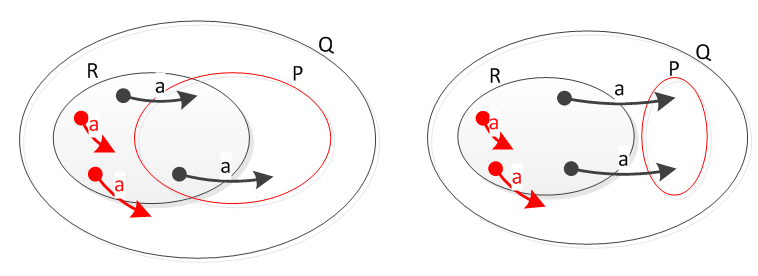
\includegraphics[width=0.8\columnwidth] {PR_1} 
	}
    \hspace{2cm}
    \subfigure[$R\cap a^{-1}P=\{q\in R|q\cdot a\in P\}$]{
    	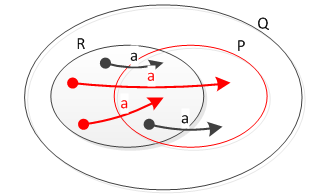
\includegraphics[width=0.4\columnwidth] {PR_2} 
    }
    \subfigure[$R\setminus a^{-1}P =\{q\in R|q\cdot a\notin P \}$]{
    	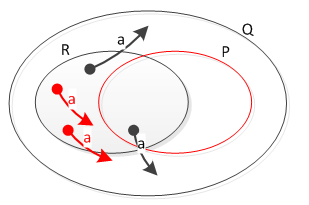
\includegraphics[width=0.4\columnwidth] {PR_3} 
    }
    \caption{$(P,a)|R=(R\cap a^{-1}P) \cup (R\setminus a^{-1}P)$}
\end{figure}

The pair $(P,a)$ is called a \textit{splitter}. Observe that $(P,a)|R=\{R\}$ if either $R\cdot a\subset P$ or $R\cdot a\cap P=\emptyset$, and $(P,a)|R$ is composed of two classes if both $R\cdot a\ne\emptyset$ and $R\cdot a\cap P^c\ne\emptyset$ or equivalently if $R\cdot a\nsubseteq P^c$ and $R\cdot a\nsubseteq P$. if $(P,a)|R$ contains two classes, then we say that $(P,a)$  \textit{splits} $R$. Note that the pair $S=(P,a)$ is called a splitter even if it does not split.

It is useful to extend the notation above to words. Given a word w and sets $P,R\subset Q$ of states, we denote by $w^{-1}P$ the set of states such that $q\cdot w\in P$, and by $(P,w)|R$ the partition of $R$ composed of the nonempty sets among
\[R\cap w^{-1}P=\{q\in R|q\cdot w\in P \} \text{ and } R\setminus w^{-1}P=\{q\in R |q\cdot w\notin P \} \]

As an example, the partition $(F,w)|Q$ is the partition of $Q$ into the set of those states from which $w$ is accepted, and the other ones. A state $q$ in one of the sets and a state $q^\prime$ in the
other are sometimes called \textit{separated} by $w$.

The Nerode equivalence is the coarsest equivalence relation on the set of states that is a (right) congruence saturating $F$. With the notation of splitters, this can be rephrased as follows.

We use later the following lemma which is already given in Hopcroft’s paper [\cite{Hopcroft71}]. It is the basic observation that ensures that Hopcroft’s algorithm works correctly.

\begin{proposition}
	The partition corresponding to the Nerode equivalence is the coarsest partition $P$ such that no splitter $(P, a)$, with $P \in \mathcal{P}$ and $a\in A$, splits a class in $\mathcal{P}$, that is	such that $(P, a)|R = \{R\}$ for all $P,R\in \mathcal{P} $and $a\in A$. $\hfill\square$
\end{proposition}

\begin{lemma}
	Let $P$ be a set of states, and let $\mathcal{P} = \{P_1, P_2\}$ be a partition of P. For any letter $a$ and for any set of states $R$, one has
	\[(P,a)|R\land (P_1,a)|R=(P,a)|R\land (P_2,a)|R=(P_1,a)|R\land (P_2,a)|R \]
	and consequntly
	\begin{align} 
	(P,a)|R \ge (P_1,a)|R\land (P_2,a)|R,\\
	(P_1,a)|R \ge (P,a)|R\land (P_2,a)|R
	\end{align}
\end{lemma}

\begin{example}
	We consider the automata given in Figure \ref{fig:revsFA} over the alphabet $A = {a, b}$.	Each automaton is the reversal of the other. However, determinization of the automaton
	on the left requires exponential time and space.
	\begin{figure}[htbp]
		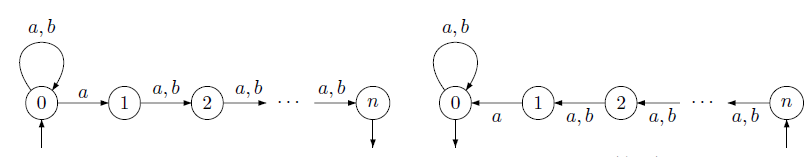
\includegraphics[scale=0.6]{revsFA}
		\caption{The automaton on the left recognizing the language $A^\ast aA^n$. It has $n + 1$ states and the minimal deterministic automaton for this language has $2^n$ states. The	automaton on the right is its reversal. It is minimal and recognizes $A^naA^\ast$.}
	    \label{fig:revsFA}
	\end{figure}
\end{example}

\subsection{Moor's algorithm}

The minimization algorithm given by Moore computes the Nerode equivalence by a stepwise refinement of some initial equivalence. All automata are assumed to be deterministic.

\begin{definition}[Moore equivalence of order $h$]
	Let $\mathcal{A}=(Q,i,F)$ be an automaton over an alphabet $A$. Define, for $q\in Q$ and $h\ge 0$, the set 
	\[L_q^{(h)}(\mathcal{A})=\{w\in A^\ast||w|\le h, q\cdot w\in F \}. \]
	The Moore equivalence of order $h$ is the equivalence $\equiv_h$ on $Q$ defined by
	\[p\equiv_h q\Leftrightarrow L_p^{(h)}(\mathcal{A})=L_q^{(h)}(\mathcal{A})\]
\end{definition}

\begin{algorithm}  
	\caption{Moore's minimization algorithm}  \label{alg:moore}
	\begin{algorithmic}%[1] %每行显示行号  
		\Require $\mathcal{A}=(Q,i,F)$  
		\Ensure The equivalence classes of $Q$  
		\State $\hat{P} \gets \{F,F^c \}$  \qquad\qquad $\triangleright$ The initial partition
		\Repeat
		\State $\hat{P}^\prime \gets \hat{P}$  \qquad\qquad $\triangleright$  $\hat{P}^\prime$ is the old partition, $\hat{P}$ is the new one
		\ForAll {$a\in A$} 
			\State $\hat{P}_a \gets \bigwedge_{P\in \hat{P}}(P,a)|Q$
		\EndFor
		\State $\hat{P}\gets \hat{P}\land \bigwedge_{a\in A}\hat{P}_a$
		\Until {$P=P^\prime$}
	\end{algorithmic}   
\end{algorithm}

The computation is described in algorithm \ref{alg:moore}. It is realized by a loop that refines the current partition. The computation of the refinement of $k$ partitions of a set swith $n$ elements can
be done in time $O(kn^2)$ by brute force. A radix sort improves the running time to $O(kn)$. With $k = Card(A)$, each tour in the loop is realized in time $O(kn)$, so the total time is $O(\mathit{l}kn)$, where $\mathit{l}$ is the number of refinement steps in the computation of the Nerode equivalence $\equiv$, that is the depth of the automaton.

The worst case behavior is obtained for $\mathit{l} = n − 2$. We say that automata having maximal depth are slow and more precisely are slow for Moore automata.

Radix sort(see, \url{https://en.wikipedia.org/wiki/Radix_sort})
In computer science, radix sort is a non-comparative integer sorting algorithm that sorts data with integer keys by grouping keys by the individual digits which share the same significant position and value.

\subsection{Hopcroft's algorithm}

Hopcroft has given an algorithm that computes the minimal automaton of a given deterministic automaton. The running time of the algorithm is $O(k n \log n)$ where $k$ the cardinality of the alphabet and $n$ is the number of states of the given automaton.

\begin{algorithm}  
	\caption{Hopcroft's minimization algorithm}  \label{alg:hopcroft}
	\begin{algorithmic}[1] %每行显示行号  
		\Require $\mathcal{A}=(Q,i,F)$  
		\Ensure The equivalence classes of $Q$  
		\State $\hat{P} \gets \{F,F^c \}$  \qquad\qquad $\triangleright$ The initial partition
		\State $W\gets \emptyset$  \qquad\qquad $\triangleright$ The waiting set
		\ForAll {$a\in A$}
			\State $ADD((min(F,F^c),a),W)$ \qquad\qquad $\triangleright$ initialization of the waiting set
		\EndFor
		\While {$W\ne\emptyset$}
			\State $(W,a)\gets TakeSome(W)$ \qquad\qquad $\triangleright$ Take and remove some splitter
			\ForAll {$P\in \hat{P}$} which is split by $(W,a)$
				\State $P^{\prime},P^{\prime\prime}\gets (W,a)|P$ \qquad\qquad $\triangleright$ Compute the split
				\State Replace $P$ by $P^\prime$ and $P^{\prime\prime}$ in $\hat{P}$ \qquad\qquad $\triangleright$ Refine the partition
			\EndFor 
			\ForAll {$b\in A$}  \qquad\qquad $\triangleright$ Update the waiting set
				\If {$(P,b)\in W$}
				  	\State Replace $(P,b)$ by $(P^\prime,b)$ and $(P^{\prime\prime})$ in $W$
				\Else
					\State $ADD((min(P^\prime,P^{\prime\prime}),b),W)$
				\EndIf  
			\EndFor
		\EndWhile
	\end{algorithmic}
\end{algorithm}

\subsubsection{Outline}

The algorithm is outlined in the function HOPCROFT given in algorithm \ref{alg:hopcroft}. We denote by $min(P, P^\prime)$ the set of smaller size of the two sets $P$ and $P^\prime$, and any one of them if they
have the same size.

Given a deterministic automaton $\mathcal{A}$, Hopcroft's algorithm computes the coarsest congruence which saturates the set $F$ of final states. It starts from the partition ${F, F^c}$ which obviously saturates $F$ and refines it until it gets a congruence. These refinements of the
partition are always obtained by splitting some class into two classes.

The algorithm proceeds as follows. It maintains a current partition $\hat{P} = {P_1,\dots,P_n}$ and a current set $W$ of splitters, that is of pairs $(W, a)$ that remain to be processed, where $W$ is a class of $\hat{P}$ and $a$ is a letter. The set $W$ is called the waiting set. The algorithm stops when the \textit{waiting} set $W$ becomes empty. When it stops, the partition $\hat{P}$ is the coarsest congruence that saturates $F$. The starting partition is the partition ${F, F^c}$ and the starting set $W$ contains all pairs $(min(F, F^c), a)$ for $a\in A$.

The main loop of the algorithm removes one splitter $(W, a)$ from the waiting set $W$ and performs the following actions. Each class $P$ of the current partition (including the class $W$) is checked as to whether it is split by the pair $(W, a)$. If $(W, a)$ does not split $P$, then nothing is done. On the other hand, if $(W, a)$ splits $P$ into say $P^\prime$ and $P^{\prime\prime}$, the class $P$ is replaced in the partition $\hat{P}$ by $P^\prime$ and $P\prime\prime$. Next, for each letter $b$, if the pair $(P, b)$ is in $W$, it is replaced in $W$ by the two pairs $(P^\prime, b)$ and $(P^{\prime\prime}, b)$, otherwise only the pair $(min(P^\prime, P^{\prime\prime}), b)$ is added to $W$.

It should be noted that the algorithm is not really deterministic because it has not been specified which pair $(W, a)$ is taken from $W$ to be processed at each iteration of the main loop. This means that for a given automaton, there are many executions of the algorithm. It turns out that all of them produce the right partition of the states. However, different executions may give rise to different sequences of splitting and also to different running time. Hopcroft has proved that the running time of any execution is bounded by $O(|A|n\log n)$.

\section{From \cite{Knuutila2001}}

\subsection{Sets,relations and mappings}

The cardinality of a set $A$ is denoted by $|A|$. 

Let $A$ and $B$ be sets and $\rho\subseteq A\times B$ a (binary) relation from $A$ to $B$. The fact that $(a,b)\in\rho (a\in A,b\in B)$ is also expressed by writing $a\rho b$. For any $a\in A$, we denote by $a\rho$ the set of elements of $B$ that are in relation $\rho$ with $a$, i.e. $a\rho=\{b\in B|a\rho b\}$. The converse of is the relation $\rho^{-1}=\{(b,a)|a\rho b\}$.Obviously $b\rho^{-1}=\{a|a\rho b\}$.

Next we consider relations on a set $A$, i.e. subsets of $A\times A$.
Theses include the diagonal relation $\omega_A=\{(a,a)|a\in A \}$, and the universal relation $\iota_A=A\times A$. The powers $\rho^n(n\ge 0)$ of a relation $\rho$ are defined as follows:
\begin{align*}
\rho^0 &=\omega_A \\
\rho^{n+1} &=\rho^n\circ \rho, \qquad n\ge 0.
\end{align*}

The relation $\rho$ is called reflexive if $\omega_A\subseteq\rho$; symmetric if $\rho^{-1}\subseteq\rho$; and transitive if $\rho^2\subseteq\rho$.

A relation on $A$ is called an \textit{equivalence relation} on $A$, if it is reflexive, symmetric and transitive. The set of all equivalence relations on a set $A$ is denoted by $Eq(A)$. It is obvious that both $\omega_A\in Eq(A)$ and $\iota_A \in Eq(A)$. Let $\rho\in Eq(A)$. The $\rho$-class $a\rho$ of an element $a (\in A)$ is also denoted by $a/\rho$. The \textit{quotient set} or the \textit{partition of A} with
respect to $\rho$, is $A/\rho=\{a\rho|a\in A \}$. If $\pi\in Eq(A)$ and $\pi\subset \rho$, then the partition $A/\pi$ is a \textit{refinement} of $A/\rho$ (each $\rho$-class is a union of some $\pi$-classes); this is also expressed by saying that $\pi$ is \textit{finer} than $\rho$ or that $\rho$ is \textit{coarser} than $\pi$. We often define an equivalence relation $\rho$ on $A$ via the set $A/\rho$, i.e. in the form $A/\rho=\{C_1,\dots,C_m \}$, where the sets $C_i$ are the classes of $\rho$.

The cardinality of $A/\rho$ is called the \textit{index} of $\rho$; especially, if $A/\rho$ is finite, then is said to have a  \textit{finite index}. For any subset $H$ of $A$, $H/\rho$ denotes $\{a\rho|a\in H \}$. The equivalence $\rho$ saturates the subset $H$, if $H$ is the union of some $\rho$-classes. Hence, $\rho$ saturates $H$ iff $a\rho\in H/\rho$ implies $a\rho\subseteq H$.

A \textit{mapping} or a \textit{function} $\phi:A\to B$ is a relation $\phi\subseteq A\times B$ such that $|a\phi|=1$ for all $a\in A$. If $a\phi b$, then $b$ is the \textit{image} of $a$ and $a$ is a \textit{preimage} of $b$. That $b$ is an image of $a$ is expressed by writing $b=\phi(a)$ and that $a$ is a preimage of $b$ is written as $a=\phi^{-1}(b)$. The notation $a=\phi^{-1}(b)$ is justified合理的, when  $\phi$  is bijective (see below). The \textit{restriction} of a mapping $\phi:A\to B$ to a set $C\subseteq  A$ is the mapping $\phi|C:C\to B$ where $\phi|C=\phi\cap(C\times B)$.

The \textit{composition} of two mappings $\phi:A\to B$ and $\psi:B\to C$ is the mapping
$\phi\psi: A\to C$, where $\phi\psi$ is the product of $\phi$ and $\psi$ as relations. The \textit{kernel} $\phi\phi^{-1}$ of a mapping $\phi:A\to B$, also denoted by $\ker\phi$, is an equivalence relation on $A$ and $a\phi\phi^{-1}b$ iff $a\phi=b\phi (a,b\in A)$. A mapping $\phi:A\to B$ is called \textit{injective} if $\ker \phi=\omega_A$; \textit{surjective} (or onto) if $A\phi =B$; and \textit{bijective} if it is both injective and surjective.

\begin{figure}[htbp]
	\subfigure[An injective non-surjectice function(injection, not a bijection) ]{
		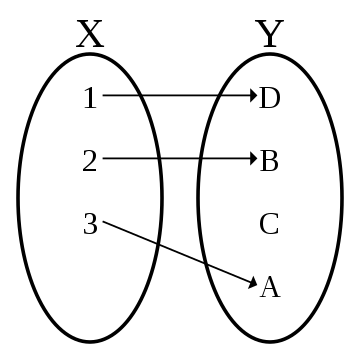
\includegraphics[width=0.2\columnwidth] {Injection} 
	}
	\subfigure[An injective surjective function (bijection) ]{
		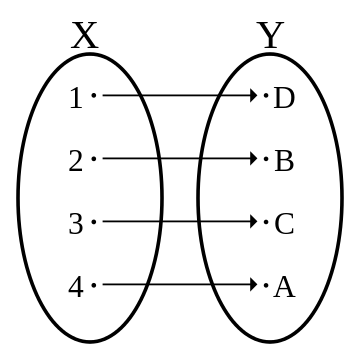
\includegraphics[width=0.2\columnwidth] {Bijection} 
	}
    \subfigure[A non-injective surjective function (surjection, not a bijection) ]{
    	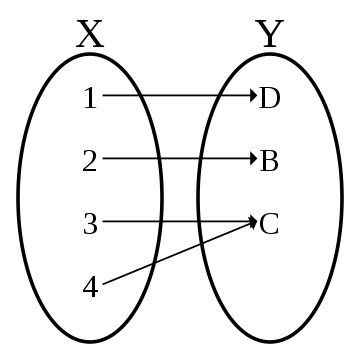
\includegraphics[width=0.2\columnwidth] {Surjection} 
    }
	\subfigure[A non-injective non-surjective function (also not a bijection) ]{
		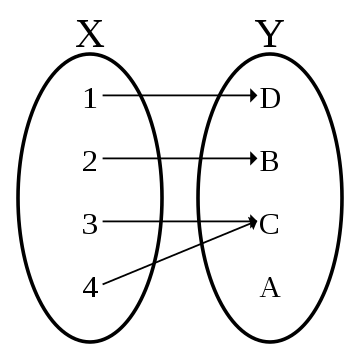
\includegraphics[width=0.2\columnwidth] {Not-Injection-Surjection} 
	}
\caption{The term one-to-one function must not be confused with one-to-one correspondence (a.k.a. bijective function), which uniquely maps all elements in both domain and codomain to each other}
\end{figure}

\subsection{Preliminaries}

\begin{definition}[$a\rho_Gb$]
	DFA $G=(Q,\Sigma,\delta,q_0,F)$, Two states $a$ and $b$ of $G$ are equivalent, which we express by writing $a\rho_G b$, if 
	\[(\forall w\in \Sigma^\ast) (\delta(a,w)\in F)\Leftrightarrow\delta(b,w)\in F) \]
\end{definition}

\begin{definition}[$\omega_Q,\iota_Q,Eq(Q)$]
	DFA $G=(Q,\Sigma,\delta,q_0,F)$, the diagonal relation $\omega_Q=\{(a,a)|a\in Q \}$, the universal relation $\iota_Q=Q\times Q$. The set of all equivalence relations on a set $Q$ is denoted by $Eq(Q)$. It is obvious that both $\omega_Q\in Eq(Q)$ and $\iota_Q \in Eq(Q)$. 
\end{definition}

\begin{definition}[the reduced $G$]
	DFA $G$ is reduced, if $a\rho_G b$ implies $a=b$, i.e. $\rho_G=\omega_Q$
\end{definition}

\begin{definition}[$Con(G)$]
	A relation $\rho\in Eq(Q)$ is a congruence of $G$, if 
	\begin{enumerate}[(1) ]
		\item $a\rho b$ implies $\delta(a,x)\rho\delta(b,x)$ for all $a,b\in Q$ and all $x\in \Sigma$, and
		\item $\rho$ saturates $F$ 
	\end{enumerate} 
	We denote by $Con(G)$ the set of all congruences of $G$. 
\end{definition}

\begin{definition}[quotient DFA $G/\rho$]
	It is well-known that the relation $\rho_G$ is the greatest (coarsest)  congruence of $G$. For any $\rho\in Con(G)$ the quotient DFA $G/\rho$ is defined as $G/\rho=(Q/\rho,\Sigma,\delta/\rho,q_0/\rho,F/\rho)$ where $\delta/\rho(a/\rho,x)=\delta(a,x)/\rho$. 
\end{definition}

\begin{definition}[DFA as unary algebras]
	DFA $G=(Q,\Sigma,\delta,q_0,F)$, $\Sigma$ is viewed as a set of unary operation symbols and the transition function $\delta$ of $G$ is replaced by the $\Sigma$-indexed family $(x^G:x\in\Sigma)$ of unary operations which are defined so that for any $x\in\Sigma$ and $a\in Q, x^G(a)=\delta(a,x)$. We shall omit $G$ from the superscript and write simply $x(a)$ for $\delta(a,x)$. 
	
	Clearly, a string $w=x_1x_2\dots x_n$ is accepted by $G$ if and only if $x_n(\dots(x_2(x_1(q_0))\dots)\in F$. 
\end{definition}

\subsection{The classical algorithm}

The classical minimization algorithm is based on the following ``layer-wise' definition for the equivalence relation $\rho_G$.

\begin{proposition} \label{pro:eq}
	Let $G=(Q,\Sigma,\delta,q_0,F)$ and a series $\rho_i (i\ge 0)$ of equivalence relations on $Q$ be defined as follows:
	\begin{align*}
	\rho_0 &=\{(a,b)|a,b\in F \} \cup \{(a,b)|a,b\in Q-F \},\\
	\rho_{i+1} &=\{(a,b)\in\rho_i|(\forall x\in \Sigma) (\delta(a,x),\delta(b,x))\in\rho_i \}
	\end{align*}
	Then the following hold.
	\begin{enumerate} [(1) ]
		\item $\rho_0\supseteq\rho_1\supseteq\cdots$
		\item If $\rho_i=\rho_{i+1}$ then $\rho_i=\rho_{i+j}$ for all $j>0$ and furthermore, $\rho_i=\rho_G$.
		\item There exists $0\le k\le |Q|$ such that $\rho_k=\rho_{k+1}$. 
	\end{enumerate}
\end{proposition}

\textbf{ The refinements on individual classes}

When the construction of Proposition \ref{pro:eq} is implemented, each refinement step leading from $\rho_i$ to $\rho_{i+1}$ consists of a series of refinements on individual classes of $\rho_i$. The refinement of a single class $B$ can be implemented with suitably chosen data structures for equivalence relations to run in time $O(|\Sigma||B|)$, and each refinement from $\rho_i$ to $\rho_{i+1}$
takes thus time $O(|\Sigma||Q|)$.

\begin{example}
	We construct (the worst kind of ) a DFA Fig. \ref{fig:mini-ex1_1}.
	
	\begin{align*}
		G/\rho_0&=\{\{6\},\{1,2,3,4,5\} \}, \\
		B &= \{1,2,3,4,5 \}, \delta(5,0)\notin B,\delta(i,0)=i+1\in B,1\le i \le 4,\\
		G/\rho_1&=\{\{6\},\{5\}, \{1,2,3,4 \} \} \\
		B &= \{1,2,3,4 \}, \delta(4,0)\notin B,\delta(i,0)=i+1\in B,1\le i \le 3,\\
		G/\rho_2&=\{\{6\},\{5\}, \{4\}, \{1,2,3\} \} \\
		B &= \{1,2,3 \}, \delta(3,0)\notin B,\delta(i,0)=i+1\in B,1\le i \le 2,\\
		G/\rho_3&=\{\{6\},\{5\}, \{4\}, \{3\},\{1,2\} \} \\
		B &= \{1,2 \}, \delta(2,0)\notin B,\delta(i,0)=i+1\in B,1\le i \le 1,\\
		G/\rho_4&=\{\{6\},\{5\}, \{4\}, \{3\},\{2\},\{1\} \} 
	\end{align*}
	
	The classical minimization algorithm is ineffective, since in the worst kind of a DFA, each refinement step from $\rho_i$ to $\rho_{i+1}$ removes always one state from the only nonsingleton class. The work performed by the algorithm (even if we optimize it to avoid considering singleton classes) will then be proportional to $|\Sigma|\sum_{i=1}^{|Q|-2}(|Q|-i)$, which leads to $O(|\Sigma||Q|^2)$ execution time.
	
	\begin{figure}[htbp]
		\begin{tikzpicture}[->,>=stealth',shorten >=1pt,auto,node distance=2cm, semithick]
		\tikzstyle{every state}=[minimum size=0.1mm]
		\node[initial,state] (p1)  {$1$};
		\node[state]         (p2) [right of=p1] {$2$};
		\node[state]         (p3) [right of=p2] {$3$};
		\node[state]         (p4) [right of=p3] {$4$};
		\node[state]         (p5) [right of=p4] {$5$};
		\node[state,accepting] (p6) [right of=p5] {$6$};
		\path
		(p1) edge [loop above] node {1} (p1)
		edge [] node {0} (p2)
		(p2) edge [loop above] node {1} (p2)
		edge [] node {0} (p3)
		(p3) edge [loop above] node {1} (p3)
		edge [] node {0} (p4)
		(p4) edge [loop above] node {1} (p4)
		edge [] node {0} (p5)
		(p5) edge [loop above] node {1} (p5)
		edge [] node {0} (p6)
		(p6) edge [loop above] node {0,1} (p6)
		;
		\end{tikzpicture}
		\caption{Minimizing example} \label{fig:mini-ex1_1}
	\end{figure}
\end{example}

\subsection{Atomic refinements}

Note that the construction of Proposition \ref{pro:eq}  reaches the situation $\rho_i = \rho_{i+1}$ when $\rho_i$ becomes a congruence, i.e. 
\[(\forall a,b\in Q, x\in Q) a\rho_i b\implies \delta(a,x)\rho_i\delta(b,x) \]. 

Now consider the situation where $\rho_i \ne \rho_{i+1}$. Obviously,
\begin{align*}
\rho_i\ne\rho_{i+1} &\Leftrightarrow (\exists a,b\in Q,x\in\Sigma) &(a,b)\in\rho_i \text{ and } (\delta(a,x),\delta(b,x))\notin\rho_i\\
&\Leftrightarrow (\exists B\in Q/\rho_i,x\in\Sigma) &(a,b)\in B  \text{ and } (\delta(a,x),\delta(b,x))\notin\rho_i\\
&\Leftrightarrow (\exists B,C\in Q/\rho_i,x\in\Sigma) &(a,b)\in B  \text{ and } \delta(a,x)\in C, \text{ and } \delta(b,x))\notin C\\
&\Leftrightarrow (\exists B,C\in Q/\rho_i,x\in\Sigma) &(a,b)\in B  \text{ and } \delta(B,x)\cap C\ne\emptyset, \text{ and } \delta(B,x))\nsubseteq C
\end{align*}

The step from $\rho_i$ to $\rho_{i+1}$ can thus be understood as a series of ``atomic' refinements performed for such $x\in \Sigma, B,C\in Q/\rho_i$ that
\begin{equation}\label{equ:atomic}
	\delta(B,x)\cap C\ne\emptyset \text{ and } \delta(B,x))\nsubseteq C
\end{equation}
holds, Each such atomic refinement partition then $B$ into $B\cap x^{-1}(C) \}$ and $B-(B\cap x^{-1}C))$. We denote these refinements of $B$ with $B_{C,x}$ and $B^{C,x}$, respectively. We use the notation $B^\prime$ and $B^{\prime\prime}$ for these refinements of $B$ when their relation to the pair $(C,x)$ has no importance.

Let us next rewrite Proposition \ref{pro:eq} in the terms of these atomic refinements.

\begin{proposition} \label{pro:eq_relations}
	Let $G=(Q,\Sigma,\delta,q_0,F)$ be a DFA and series $\theta_i (i\ge 0)$ of equivalence relation on $Q$ be defined as follows:
	\begin{align*}
		Q/\theta_0 &=\{F,Q-F \}, &\\
		Q/\theta_{i+1} &=\begin{cases}
		(Q/\theta_i-\{B\})\cup\{B_{C,x},B^{C,x}\} &\text{ if \ref{equ:atomic} holds for some } B,C\in Q/\theta_i, x\in\Sigma,\\
		Q/\theta_i &\text{otherwise}.
		\end{cases}
	\end{align*}
	Then there exists a $k\le |Q|$ such that $\theta_{i+l}=\theta_i$ for all $l\ge 0$ and $\theta_k=\rho_G$.
\end{proposition}

\begin{proof}
	The upper bound comes from the observation, that each atomic refinement increases the index of $\theta_i$ by one. Naturally this index cannot be increased more than $|Q|-1$ times.
	
	It is clear that $\theta_k$ is both an equivalence relation saturating $F$ (it is a refinement of $\theta_0$) and a congruence of $G$ (since Eq. (\ref{equ:atomic}) does not hold for $\theta_k$). What remains, is to show that $\theta_k$ is also the \textit{greatest} congruence $\rho_G$ of $G$.
	
	We show first that $\theta_i\supseteq\rho_G$ for all $i\ge 0$. When contraposed, the claim is that if $(a,b)\notin\theta_i$ then $(a,b)\notin\rho_G$ (for all $i\ge 0$). This is clearly true for $\theta_0$, since final and non-final states are not in $\rho_G$. Suppose then that the claim holds for all $0\le l\le i$ and let $(a,b)\in\theta_i$. If $(a,b)\notin\theta_{i+l}$, it must be the case that for some $x\in\Sigma,(x(a),x(b))\notin\theta_i $. 
	But this implies (by IA) that $x(a)$ and $x(b)$ are not in $\rho_G$. Thus, $a$ and $b$ become inequivalent in $\theta_{i+l}$ only when they are shown to be inequivalent in $\rho_G$, formally $(a,b)\notin\theta_{i+l}\implies (a,b)\notin\rho_G$. 
	
	It now holds that $\theta_0\supseteq\theta_1\supseteq\cdots\supseteq\theta_k$ (by definition), and consequently $\theta_0\supseteq\theta_1\supseteq\cdots\supseteq\theta_k\supseteq\rho_G$. Since $\rho_G$ is the greatest congruence of $G$, and $\theta_k$ is a congruence, it must be the case that $\theta_k=\rho_G$.  $\hfill\square$.
\end{proof}

Note that the construction given in Proposition \ref{pro:eq_relations} does not fix the order in which the triples $B, C, x$ are exploited to refine $\theta_i$. Thus, all the different orderings yield the same result at the end: the unique greatest congruence.

\begin{algorithm}  
	\caption{Comuting $\rho_G$ using atomic refinements}  \label{alg:atomic}
	\begin{algorithmic}[1] %每行显示行号  
		\Function {Equivalence} {$G$}
		\State $Q/\theta\gets \{F,Q-F\}$
		
		\While {($\exists B,C\in Q/\theta,x\in\Sigma$ s.t. Eq. \ref{equ:atomic} holds)}
		\State $Q/\theta\gets(Q/\theta-\{B\}\cup\{B_{C,x},B^{C,x}  \}$
		\EndWhile
		
		\State \Return{$\theta$}  
		\EndFunction 
	\end{algorithmic}
\end{algorithm}

How to efficiently find some triple $B,C,x$ for which Eq. (\ref{equ:atomic}) holds.

The refiners of $B$ in $\theta$, shortly $ref(B,\theta)$:
\[ref(B,\theta)=\{(C,x)\in(Q/\theta)\times\Sigma|x(B)\cap C\ne\emptyset \text{ and } x(B)\nsubseteq C \} \]

As each $B$ is related to $ref(B,\theta)$, so is each pair $(C,x)$ related to its \textit{objects of refinement} in $\theta$,
\[obj(C,x,\theta)=\{B\in Q/\theta|(C,x)\in ref(B,\theta) \} \]

\begin{algorithm}  
	\caption{Refiner-driven implementation}  \label{alg:refiner-driven}
	\begin{algorithmic}[1] %每行显示行号  
		\Function {Equivalence} {$G$}
		\State $Q/\theta\gets \{F,Q-F\}$
		
		\While {($\exists some(C,x)\in(Q/\theta)\times\Sigma$ with $obj(C,x,\theta)\ne\emptyset$)}
		\For {$B\in obj(C,x,\theta)$}
			\State replace $B$ with $B_{C,x}$ and $B^{C,x}\in Q/\theta$
		\EndFor
		\EndWhile
		
		\State \Return{$\theta$}  
		\EndFunction 
	\end{algorithmic}
\end{algorithm}

\begin{lemma} \label{lemma:refine_B}
	Let $G=(Q,\Sigma,\delta,q_0,F),\theta\in Eq(Q)$ and $B,C\in Q/\theta$ and $x\in\Sigma$. Suppose we refine $B\in Q/\theta$ into $B_{C,x}$ and $B^{C,x}$ with respect to $(C,x)$. Let $D$ be a subset of $B_{C,x}$ or $B^{C,x}$, then $D\notin(C,x,\theta)$.
\end{lemma}

\begin{proof}
	Let us first condider the case $D\in\{B_{C,x},B^{C,x}\}$. Then either $x(a)\in C$ for all $a\in D$ or $x(a)\notin C$ for all $a\in D$. The same property holds naturally for all subsets of $D$.
\end{proof}

The bookkeeping needed for telling whether a particular pair $(C,x)$ has been used can be implemented as follows:
\begin{itemize}
	\item We maintain a set $L$ of candidate refiners, shortly candidates, in $(Q/\theta)\times\Sigma$. Initially $L=\{F,Q-F\}\times X$.
	\item Pairs $(C,x)$ are now selected from $L$, not (blindly) from all of $(Q/\theta)\times\Sigma$.
	\item Every time we select a pair $(C,x)$ from $L$, we remove it from $L$. This is justified by Lemma \ref{lemma:refine_B}.
	\item After refining $\theta$ to $\theta^\prime$, we must also update $L$ to contain only classes of $\theta^\prime$. We do the following for each $x\in\Sigma$ and each class $B$ refined to $B^\prime$ and $B^{\prime\prime}$:
	\begin{itemize}
		\item[$\circ$] if $(B,x)\in L$, we remove $(B,x)$ and add both $(B^\prime,x) and (B^{\prime\prime},x)$ to $L$. This is (indirectly) justified by Proposition \ref{pro:eq_relations}, since only the current $\theta$-classes are used in the construction.	
		\item[$\circ$] If $(B,x)\notin L$, we simply add $(B^\prime)$ and $(B^{\prime\prime})$ to $L$.
	\end{itemize}
\end{itemize}

Note that new items are inserted into $L$ only when some class gets refined. Thus, $L$ will eventually become empty, because each iteration removes one element from $L$, and the total number of elements added into $L$ is bounded by $2|\Sigma||Q|$ (the maximum number of different equivalence classes created in any refinement sequence is $2|Q|-1$. The ideas above are collected into Algorithm \ref{alg:set-driven}.

\begin{algorithm}  
	\caption{Set-driven implementation}  \label{alg:set-driven}
	\begin{algorithmic}[1] %每行显示行号  
		\Function {Equivalence} {$G$}
		\State $Q/\theta\gets \{F,Q-F\}$
		\State $L\gets (Q/\theta)\times\Sigma$
		
		\While {$L\ne\emptyset$}
		\State remove a pair $(C,x)$ from $L$
		\ForAll {$B\in obj(C,x,\theta)$}
			\State replace $B$ with $B_{C,x}$ and $B^{C,x}$ in  $Q/\theta$
			\ForAll {$y\in\Sigma$}
				\If {$(B,y)\in L$}
					\State replace $(B,y)$ with $(B^\prime,y)$ and $(B^{\prime\prime},y)$ in $L$
				\Else
					\State insert $(B^\prime,y)$ and $(B^{\prime\prime},y)$ to $L$
				\EndIf
			\EndFor
		\EndFor
		\EndWhile
		
		\State \Return{$\theta$}  
		\EndFunction 
	\end{algorithmic}
\end{algorithm}

\begin{lemma} \label{lemma:refine}
	Let $G=(Q,\Sigma,\delta,q_0,F),\theta\in Eq(Q)$ and $B\in Q/\theta$. Suppose we refine $B$ into $B^\prime$ and $B^{\prime\prime}$. Then, for any $y\in\Sigma$, refining all the classes of $\theta$ with respect to any two of the pairs $(B,y),(B^\prime,y)$ and $(B^{\prime\prime})$ gives the same result as refining them with respect to all three of them.
\end{lemma}

\begin{proof}
	Consider an arbitrary class $D\in Q/\theta, a\in D$ and $y\in\Sigma$. As seen in Fig. \ref{fig:refine}, the transition $\delta(a,y)$ satisfies exactly one of the following: 
	\begin{enumerate}[(1) ]
		\item $\delta(a,y)\in B^\prime$
		\item $\delta(a,y)\in B^{\prime\prime}$
		\item $\delta(a,y)\notin B$
	\end{enumerate}
	Now each possible refinement sequence with respect to any two of the sets $B,B^\prime$ and $B^{\prime\prime}$ and letter $y$ partitions $D$ into $D_1,D_2,D_3$, which is the same as the result yielded by performing all the three refinements.
\end{proof}

\begin{figure}[htbp]
	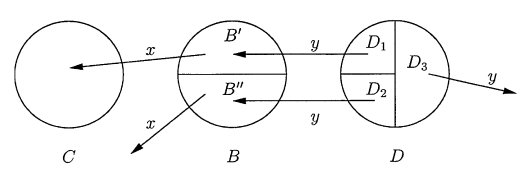
\includegraphics[scale=0.6]{refine}
	\caption{Illustration of Lemma \ref{lemma:refine}}
	\label{fig:refine}
\end{figure}

%%%%%%%%%%%%%%%%%%%%%%%%%%%%%%%%%%%%%%%%%%%%%%%%%%
\begin{thebibliography}{99}
	\bibitem[Hopcroft71]{Hopcroft71}
	Hopcroft, J.E. \textit{An n log n algorithm for minimizing states in a finite automaton}, in The Theory of Machines and Computations (Z. Kohavi, ed.), pp.180-196, Academic Press, New York, 1971.
	
	\bibitem[Gries73]{Gries73}
	Gries, D. \textit{Describing an Algorithm by Hopcroft}, Acta Inf. 2:97 109, 173. $\copyright$ by Springer-Verlag 1973
	
	\bibitem[Knuutila2001]{Knuutila2001}
	Knuutila, T. \textit{Re-describing an Algorithm by Hopcroft}. Theoret. Computer Science 250 (2001) 333--363.
		
	\bibitem[Ratnesh95]{Ratnesh95}
	Ratnesh Kumar, \textit{Modeling and Control of Logical Discrete Event Systems}, $\copyright$ 1995 by Springer Science+Business Media New York.
	
	\bibitem[Jean2011]{Jean2011}
	Jean Berstel, Luc Boasson, Olivier Carton, Isabelle Fagnot
	, \textit{Minimization of automata}, Universit$\acute{e}$ Paris-Est Marne-la-Vall$\acute{e}$e 2010 Mathematics Subject Classification: 68Q45, 2011.
	
	\bibitem[Kenneth2012]{Kenneth2012}
	Kenneth H. Rosen著,徐六通译, \textit{离散数学及其应用Discrete Mathematics and Its Applications},seventh Edition, 2012, 机械工业出版社, 北京, 2014.
	
\end{thebibliography}
